\documentclass[12pt,a4paper]{report}

% --- Paquetes de Idioma y Codificación ---
\usepackage[utf8]{inputenc}
\usepackage[T1]{fontenc}
\usepackage[spanish, es-tabla]{babel}

% --- Diseño de Página ---
\usepackage{geometry}
\geometry{top=2.5cm, bottom=2.5cm, left=3cm, right=3cm}

% --- Matemáticas y Símbolos ---
\usepackage{amsmath, amssymb, amsthm}

% --- Colores y Cajas ---
\usepackage[dvipsnames]{xcolor}
\usepackage[most]{tcolorbox}

% Caption

\usepackage{caption}

% Gráficos

\usepackage{graphicx}

% Espaciadora

\newcommand{\esp}{\vspace{0.5cm}}

% promedio

\newcommand{\prom}[1]{\left\langle #1 \right\rangle}

% ket

\newcommand{\ket}[1]{| #1 \rangle}

% bra

\newcommand{\bra}[1]{\langle #1 |}

% braket

\newcommand{\braket}[2]{\langle #1 | #2 \rangle}

% Bibliografía

\usepackage[style=apa, backend=biber]{biblatex} % Estilo APA
\addbibresource{biblio.bib} % Nombre de tu archivo .bib

% Configuración de cajas personalizadas
\newtcolorbox{importante}{
	colback=red!5!white,
	colframe=red!75!black,
	title=Importante,
	fonttitle=\bfseries
}

\newtcolorbox{nota}{
	colback=blue!5!white,
	colframe=blue!75!black,
	title=Nota,
	fonttitle=\bfseries
}

% Definición de la caja de bibliografía
\newtcolorbox{bibliografia}{
	colback=gray!5!white,
	colframe=gray!75!black,
	title=Bibliografías útiles,
	fonttitle=\bfseries,
	breakable
}

% Socrative para óptica 2

\newtcolorbox{Socrative}{
	colback=orange!5!white,
	colframe=orange!75!black,
	title=Socrative,
	fonttitle=\bfseries,
	breakable
}

% Float

\usepackage{float}

% --- Hipervínculos ---
\usepackage{hyperref}
\hypersetup{
	colorlinks=true,
	linkcolor=blue,
	filecolor=magenta,      
	urlcolor=cyan,
}

% --- Datos del Documento ---
\title{Óptica II}
\author{Chengyu Jin}
\date{\today}

\begin{document}
	
	\maketitle
	
	\tableofcontents
	\newpage
	
	\chapter{Óptica No Lineal}
	
	\section{Introducción}
	
	\begin{figure}[H]
		\centering
		
\includegraphics[width=0.7\textwidth]{IMG/intro.png}
	\end{figure}
	
	\esp
	
	\begin{figure}[H]
		\centering
		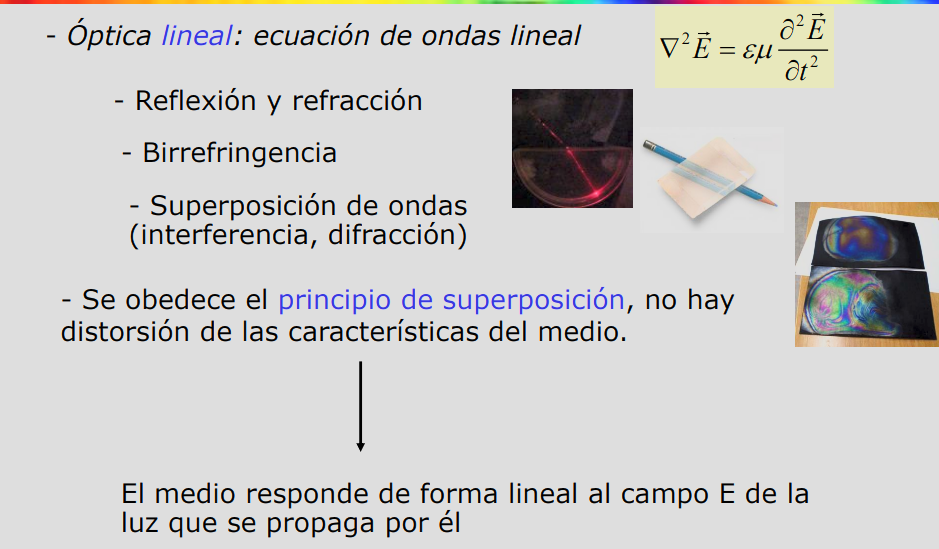
\includegraphics[width=0.7\textwidth]{IMG/intro2.png}
	\end{figure}
	
	\esp
	
	Hasta ahora, en todos los temas anteriores hemos considerado una respuesta lineal del medio por el que se propaga una onda e.m. al campo eléctrico aplicado. Como vimos en Óptica I, esto se traduce en una ecuación de ondas lineal para la amplitud de campo eléctrico (es decir, que no incluye términos de orden superior a la unidad en $\vec{E}$). Con la suposición de linealidad para el medio por el que se propaga la onda, podemos describir de forma bastante satisfactoria fenómenos de propagación como reflexión, refracción, birrefringencia natural y (considerando el principio de superposición), también los fenómenos de interferencia y difracción que hemos visto en Óptica I y en los primeros temas de Óptica II. El índice de refracción y el coeficiente de absorción no dependen de la intensidad de la onda, y la distribución en frecuencias de la onda no se modifica al propagarse por el medio.
	
	\esp

	\begin{figure}[H]
		\centering
		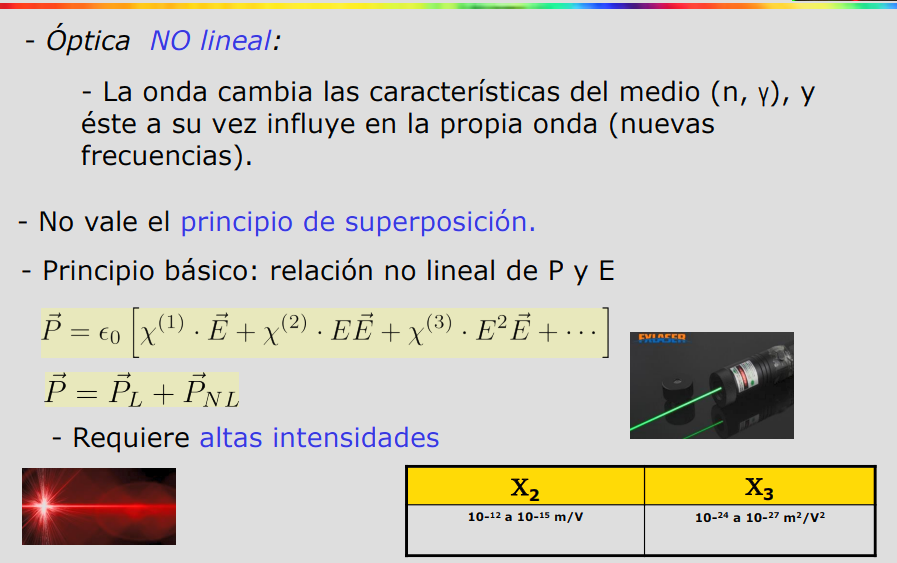
\includegraphics[width=0.7\textwidth]{IMG/intro3.png}
	\end{figure}
	
	\esp
	
	Sin embargo, con esta asunción de medios lineales hemos dejado fuera un conjunto muy amplio de fenómenos que se producen en medios donde hay una respuesta no lineal al campo eléctrico aplicado, que se manifiesta fundamentalmente cuando la intensidad de la onda que se propaga es elevada, con valores de amplitud de campo eléctrico del orden de $10^5$ a $10^8$ V/m, e irradiancias del orden de $10^8$ a $10^{12}$ W/m$^2$. La respuesta no lineal se articula principalmente a través de la dependencia del vector polarización $\vec{P}$ con el campo eléctrico, que podrá empezar a incluir términos de mayor orden en $\vec{E}$. Utilizando de forma preliminar el modelo de oscilador armónico acoplado, podemos entender cómo surge este comportamiento no lineal si consideramos que la fuerza externa va a tener una magnitud algo más próxima a las fuerzas atómicas (que suelen ser del orden de $10^{11}$ V/cm), y la fuerza compensatoria ya no sigue la ley de Hooke y es proporcional a $x$, sino que incluye términos de orden superior. El oscilador pasa a ser entonces no armónico, y esto induce una dependencia de la solución del oscilador que no es lineal con $\vec{E}$, y también a su vez induce una dependencia no lineal de la polarización con el campo eléctrico de la onda que se propaga por el medio. Si recordamos que la polarización es, según este modelo simplificado, el producto de la densidad de dipolos por unidad de volumen por la polarización de cada dipolo individual ($\vec{P} = N\vec{p}$), entonces podemos ver que la no linealidad que aparezca en el medio puede tener su origen tanto en $N$ (si la densidad de dipolos depende del campo aplicado, lo que puede suceder por ejemplo en algunos láseres) como en $\vec{p}$. Veamos entonces cómo quedaría la relación entre la polarización y la intensidad de campo eléctrico para medios no lineales, si consideramos además que en general las interacciones no lineales suelen ser bastante débiles, por lo que puede desarrollarse en serie $P$ en función de $E$:
	
	\esp
	
	\begin{equation}
		\vec{P} = \epsilon_0 \chi^{(1)} \cdot \vec{E} + \epsilon_0 \chi^{(2)} \cdot \vec{E}\vec{E} + \epsilon_0 \chi^{(3)} \cdot E^2 \vec{E} + \dots
	\end{equation}
	
	\esp
	
	\begin{figure}[H]
		\centering
		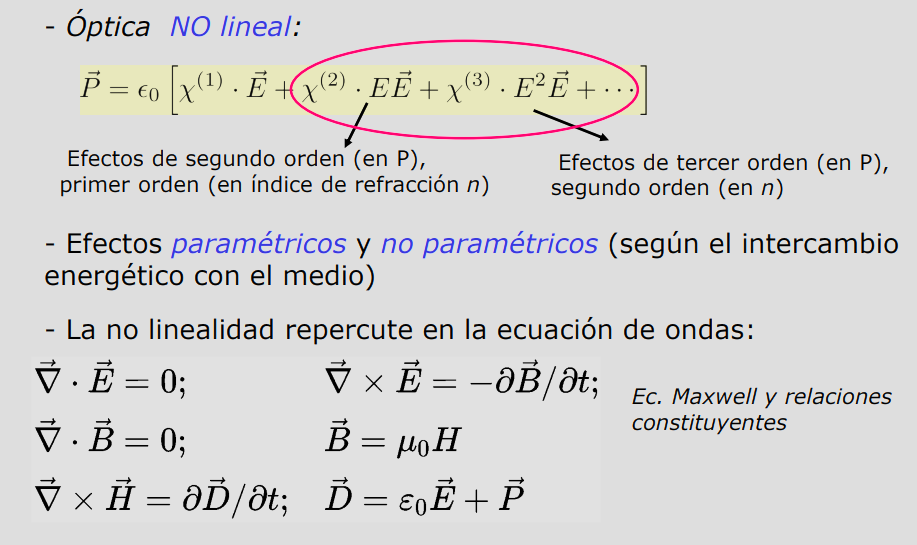
\includegraphics[width=0.7\textwidth]{IMG/intro4.png}
	\end{figure}
	
	\esp
	
	El primer término será el que predomine cuando la intensidad de la onda sea pequeña, y el medio se comportará de forma lineal, como podemos ver en la figura 1. El segundo término (potencia par de $E$) dará lugar a las interacciones no lineales de segundo orden, y su coeficiente será proporcional a la primera derivada parcial de $P$ con respecto a $E$ evaluada en $E = 0$; el siguiente término dará lugar a las interacciones de tercer orden, y será proporcional a la segunda derivada parcial de $P$ con respecto a $E$ evaluada en $E = 0$. Los valores típicos del coeficiente del término de segundo orden oscilan entre $10^{-12}$ y $10^{-15}$ m/V; los valores típicos para el coeficiente del término de tercer orden están entre $10^{-24}$ y $10^{-27}$ m$^2$/V$^2$, con lo cual se entiende claramente que sean necesarias intensidades altas para poder observar los fenómenos no lineales.

	\esp
	
	Otra clasificación posible es en interacciones o efectos \textit{paramétricos} (sin intercambio de energía con el medio, y sin alterar el estado cuántico de los átomos o moléculas del medio, como por ejemplo la generación del segundo armónico y todos los procesos que veremos a lo largo del tema) y \textit{no paramétricos} (que suceden mediante el intercambio energético con el medio y alteran los estados atómicos o moleculares, de forma que los fotones involucrados no conservan la energía porque parte de su energía puede ser traspasada al medio, o bien puede haber traspaso de energía del medio a los fotones).
	
	\esp
	
	Puede expresarse entonces $\vec{P}$ como suma de dos componentes, una lineal ($\vec{P}_L$) y otra no lineal que contiene los términos de orden superior a la unidad ($\vec{P}_{NL}$).
	
	\esp
	
	\begin{equation}
		\vec{P} = \vec{P}_L + \vec{P}_{NL}
	\end{equation}
	
	\esp
	
	\begin{figure}[H]
		\centering
		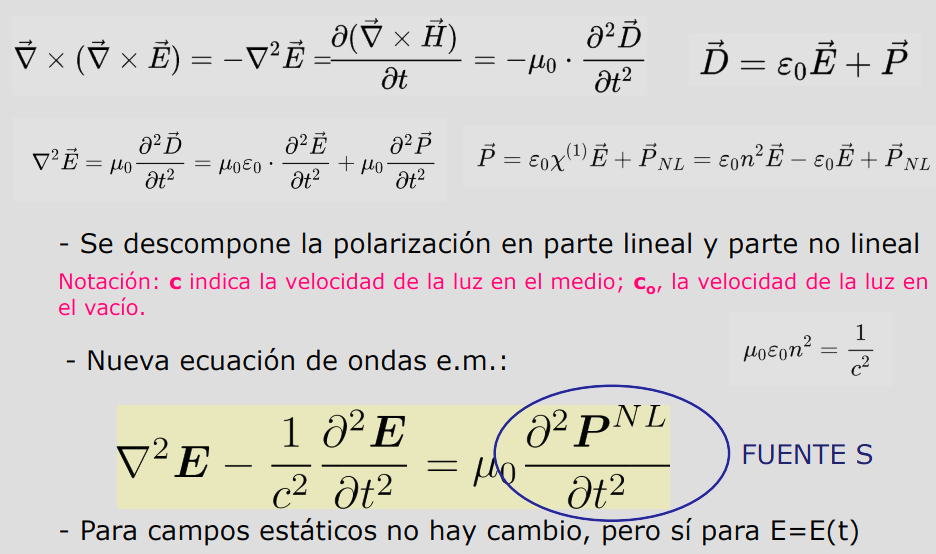
\includegraphics[width=0.7\textwidth]{IMG/intro5.png}
	\end{figure}
	
	\esp
	
	La variación de $\vec{P}$ con el tiempo hace que aparezcan nuevos términos también en la ecuación de ondas e.m., que queda de la siguiente forma:
	
	\esp
	
	\begin{equation}
		\nabla^2 E - \frac{1}{c^2} \frac{\partial^2 E}{\partial t^2} = \mu_0 \frac{\partial^2 P^{NL}}{\partial t^2}
	\end{equation}
	
	\esp
	
	La deducción de esta ecuación es similar a la vista en Óptica I, pero teniendo en cuenta la relación constituyente entre $\vec{D}$ y $\vec{E}$ en términos de $\vec{P}$: $\vec{D} = \epsilon \vec{E} + \vec{P}$. Debido a la dependencia de $\vec{P}^{NL}$ con $E$, la ecuación de ondas pasa a ser una ecuación diferencial no lineal en derivadas parciales.
	
	\esp
	
	Una consideración importante a tener en cuenta en este punto es si el campo eléctrico que provoca la respuesta no lineal es estático o bien se trata de una onda electromagnética. Para campos estáticos, la polarización sería constante, y el término adicional de la ecuación de ondas se anula. Sin embargo, en este caso el desarrollo de $\chi$ (relacionado con el cuadrado del índice de refracción) en función de potencias del campo eléctrico lleva a una dependencia del propio índice de refracción con potencias del campo eléctrico, con lo cual la no linealidad del medio se traduce en cambios del índice de refracción (y por tanto del camino óptico al recorrer el medio una onda de luz) que dependen del campo estático aplicado. Describiremos un pequeño ejemplo de este caso con campo magnético (efecto Faraday) en la primera parte del tema.
	
	\esp
	
	Sin embargo, si el campo aplicado varía con el tiempo (caso de ondas de luz de intensidad elevada), entonces sí que hay un segundo término diferente de cero en la ecuación de ondas, que se puede interpretar como una fuente de radiación secundaria generada por el propio medio al propagarse por él la onda electromagnética. Este caso lo trataremos en la segunda parte del tema.
	
	\esp
	
	Hay dos planteamientos básicos para resolver la ecuación de ondas no lineal: el primero se basa en el método iterativo de Born, y es el que describiremos con mayor profundidad en el tema. El segundo es más complejo y se conoce como teoría de ondas acopladas. Resulta útil para describir fenómenos de óptica no lineal en los cuales no puede despreciarse la interacción entre las diferentes ondas que se propagan por el medio.
	
	\esp
	
	Vamos a estudiar someramente algunas de las características más relevantes de las aplicaciones derivadas de la óptica no lineal. Como hemos visto en la primera parte de la sección, nos vamos a centrar en un tratamiento clásico derivado de la teoría electromagnética, que resulta válido para caracterizar interacciones no resonantes y no lineales con el medio (es decir, que consideraremos medios que no sean muy absorbentes). Nos referiremos exclusivamente a la respuesta no lineal de estos medios a fuentes de origen externo, como campos eléctricos o magnéticos (estos últimos sólo si son estáticos), aunque también se pueden generar efectos no lineales debido a variaciones de densidad locales por esfuerzos o tensiones aplicados.
	
	\esp
	
	\begin{figure}[H]
		\centering
		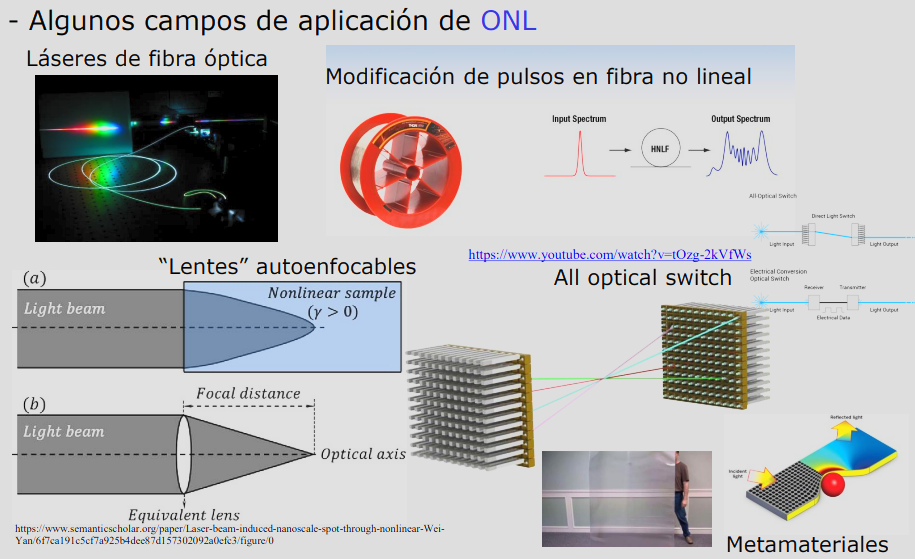
\includegraphics[width=0.7\textwidth]{IMG/intro6.png}
	\end{figure}
	
	\esp
	
	En definitiva, veremos una serie de fenómenos y aplicaciones de los mismos que surgen como consecuencia de la relación no lineal entre $\vec{P}$ y $\vec{E}$. Esto va a determinar un cambio en las características del medio por el que se propaga la onda e.m., y a su vez puede afectar a la propia onda en cuanto a su distribución en frecuencias o la cantidad de energía intercambiada o traspasada al medio. Algunos ejemplos de muestra de aplicaciones de Óptica No Lineal son los láseres de fibra óptica, que generan pulsos gracias a la amplificación en una fibra, y pueden ser sintonizables en frecuencia; las fibras no lineales que alteran selectivamente la forma de los pulsos que transmiten; las lentes autoenfocables en circuitos de fibra óptica; los interruptores \textit{all-Optical} que ahorran el paso de conversión de la señal óptica a eléctrica para el manejo de pulsos y re-distribución de señales en circuitos de telecomunicaciones, y los metamateriales, con muchas aplicaciones no sólo ópticas sino también derivadas de sus interesantes propiedades mecánicas (por ejemplo, se puede esconder un objeto también para el tacto, recubriéndolo de un metamaterial mecánico). El hecho de que la luz pueda modificarse de forma \textit{programable} a su paso por un determinado material, dependiendo de las características de la propia onda (la luz modifica a su vez a la propia luz utilizando las características del medio) abre muchísimas posibilidades de uso, y hace que este campo sea muy activo en cuanto a la investigación desarrollada desde hace ya décadas. Hay que aclarar aquí que también pueden tener lugar efectos no lineales cuando se apliquen campos eléctricos o magnéticos estáticos o casi-estáticos de elevada intensidad, y que se traducen en una variación del índice de refracción o en una birrefringencia inducida en el medio, aunque este caso no lo cubramos para campos eléctricos en el tema.
	
	\esp
	
	En las próximas secciones, veremos un ejemplo de interacción no lineal con campo estático de primer orden, y posteriormente algunos casos típicos de interacciones luz-materia no lineales (es decir, campos no estáticos), correspondientes a efectos de segundo y de tercer orden.
	
	\section{Efectos no lineales con campos estáticos}
	
	\begin{figure}[H]
		\centering
		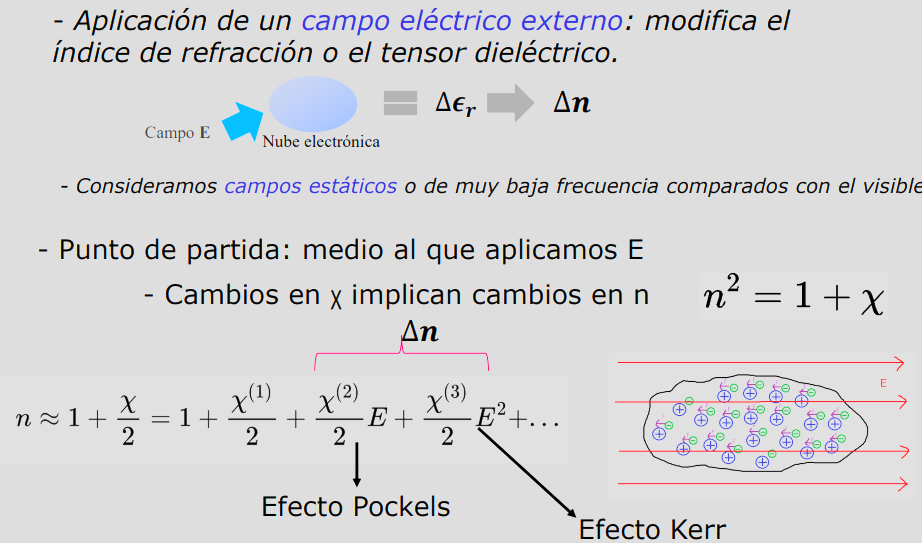
\includegraphics[width=0.7\textwidth]{IMG/efectos.png}
	\end{figure}
	
	\esp
	
	Cuando aplicamos un campo estático (o modulado con una frecuencia temporal muy baja) en determinados medios que presentan respuesta no lineal, la susceptibilidad eléctrica varía en función del campo aplicado, y por tanto se inducen también variaciones en el índice de refracción del medio:
	
	\esp
	
	\begin{equation}
		n = n_o + aE + bE^2
	\end{equation}
	
	\esp
	
	El primer término corresponde a una dependencia lineal del índice de refracción con el campo externo aplicado, y da lugar al llamado \textit{efecto Pockels}. El segundo término (dependencia cuadrática de $n$ con $E$) da lugar al \textit{efecto Kerr}. 
	
	\esp
	
	\begin{figure}[H]
		\centering
		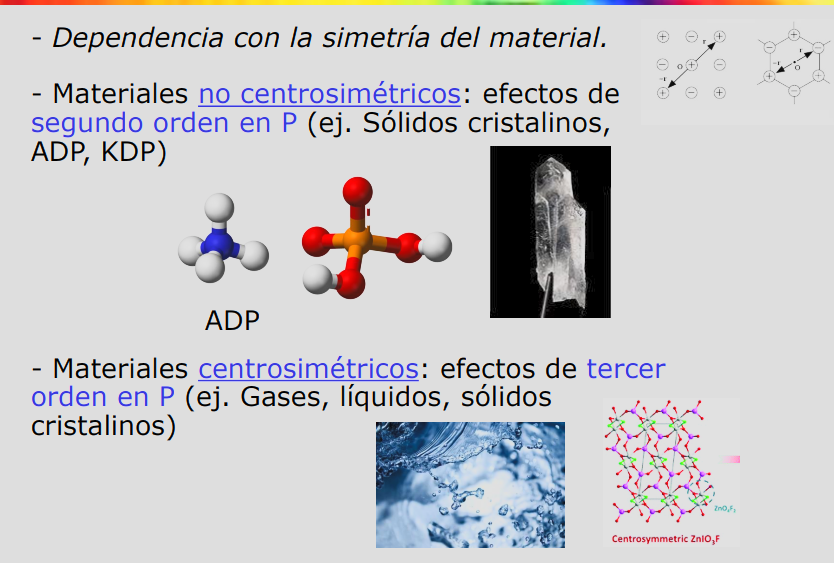
\includegraphics[width=0.7\textwidth]{IMG/efectos2.png}
	\end{figure}
	
	\esp
	
	Ambos efectos no pueden darse simultáneamente en un mismo material, porque los efectos de primer orden en $n$ (segundo orden en $P$) necesitan que el material no sea centrosimétrico. Si el material es centrosimétrico, entonces para cada punto en una posición $\vec{r}$, existe otro punto localizado del material en una posición $-\vec{r}$, es decir, hay un centro de simetría. Esto implica que el valor de sus propiedades (entre ellas, el índice de refracción) debe ser idéntico para los puntos en las posiciones $\vec{r}$ y $-\vec{r}$. Dado que $\vec{E}$ es un vector polar, es decir, que cambia de signo ante una inversión del vector $\vec{r}$, necesitamos entonces compensar este cambio de signo del vector $\vec{E}(-\vec{r})$ con potencias pares de $\vec{E}$ en el desarrollo de $n$, para que $n$ pueda mantenerse con el mismo valor en las posiciones $\vec{r}$ y $-\vec{r}$ (o sea, si $E$ cambia de signo, $E^2$ no cambia de signo, y por tanto $n$ sería idéntico en las posiciones $(\vec{r})$ y $-\vec{r}$). Por tanto, para los materiales centrosimétricos, no puede haber efectos de cambio de índice de refracción con potencias impares de $E$ (es decir, efectos de segundo orden en $P$, o primer orden en $n$).
	
	\esp
	
	Los efectos de segundo orden en $n$ (tercer orden en $P$) se dan en materiales tanto centrosimétricos como no centrosimétricos, aunque en los no centrosimétricos los efectos de primer orden predominan sobre los de segundo orden.
	
	\esp
	
	Veremos a continuación una breve descripción de un efecto de segundo orden en $\vec{P}$ relacionado con aplicación de campo magnético, con algunas de sus aplicaciones.
	
	\subsection{Efecto Faraday}
	
	\begin{figure}[H]
		\centering
		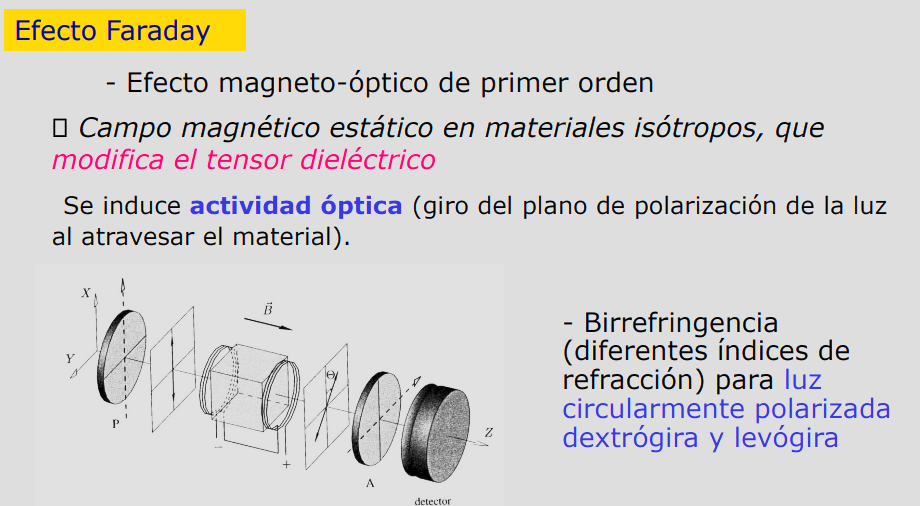
\includegraphics[width=0.7\textwidth]{IMG/fara.png}
	\end{figure}
	
	\esp
	
	El efecto Faraday es un efecto de primer orden en $n$, pero de tipo magnético. Además, la variación de índices de refracción introducida para medios inicialmente isótropos sucede en forma de birrefringencia inducida para luces circularmente polarizadas (actividad óptica). La birrefringencia inducida sería entonces proporcional al campo magnético aplicado:
	
	\esp
	
	\begin{equation}
		\Delta n = n_L - n_D = aB
	\end{equation}
	
	\esp
	
	Como se trata de un medio isótropo, ya no afectan las consideraciones de simetría explicadas para el efecto electro-óptico.
	
	\esp
	
	\begin{figure}[H]
		\centering
		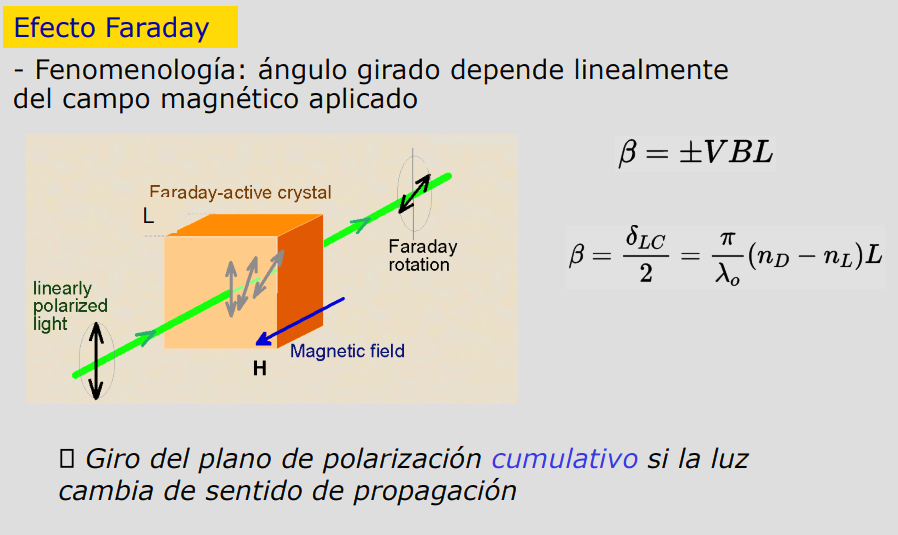
\includegraphics[width=0.7\textwidth]{IMG/fara2.png}
	\end{figure}
	
	\esp
	
	De otra forma, podemos decir que en determinados medios, el campo magnético aplicado induce actividad óptica. Experimentalmente, se encuentra que cuando incide luz linealmente polarizada propagándose en la misma dirección que el campo aplicado (configuración longitudinal), el ángulo que rota a la salida del material ($\beta$) es proporcional a la longitud de material recorrido y al campo $B$ (inducción magnética) aplicado. La constante de proporcionalidad $V$ se denomina constante de Verdet. Ya sabemos por Óptica I que el ángulo $\beta$ es justo la mitad del desfase introducido debido al efecto de birrefringencia inducido en el material, y por tanto no sorprende que
	
	\esp
	
	\begin{equation}
		\beta = \pm VBL = \frac{\delta_{LD}}{2}
	\end{equation}
	
	\esp
	
	siendo $L$ la distancia recorrida en el interior del medio. El signo más o menos que hemos introducido indica (para constante de Verdet positiva) que si la luz se propaga en el mismo sentido que el campo aplicado, el giro será dextrógiro, u horario, mientras que si se propaga en sentido opuesto a B, el giro será levógiro o antihorario. Para determinar el sentido de giro, miramos siempre la luz viniendo hacia nosotros en el sentido de propagación. Esto supone que si la luz atraviesa una vez una determinada longitud de material con efecto Faraday, se refleja y vuelve a atravesar el material, el giro con respecto a la dirección de vibración inicial es acumulativo (al cambiar el sentido de propagación, un giro levógiro equivale a uno dextrógiro en el sentido inicial).
	
	\esp
	
	En realidad, los valores de $V$ suelen ser bastante pequeños, con lo cual el valor del ángulo girado por cada $mm$ recorrido en el medio también es pequeño. Y también dependen de la longitud de onda, como se comprueba en la práctica de laboratorio sobre Efecto Faraday.
	
	\esp

	\begin{figure}[H]
		\centering
		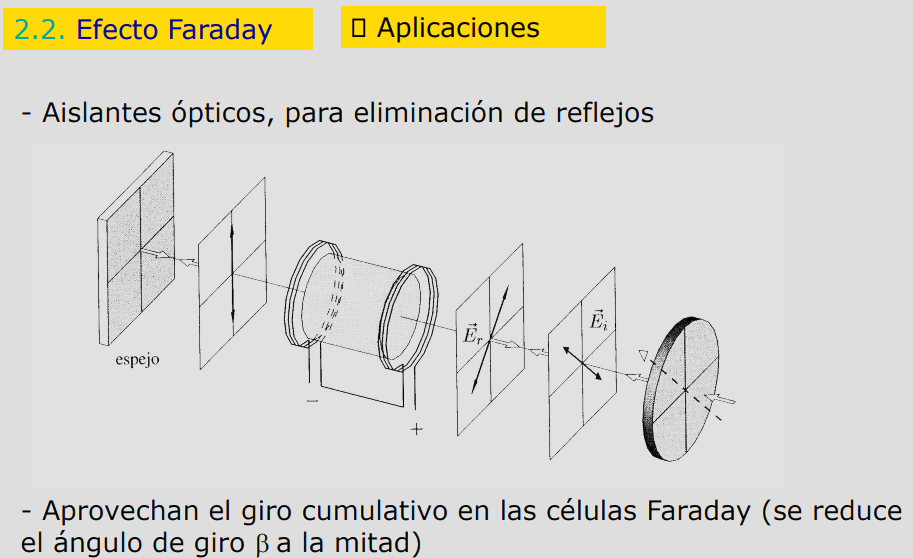
\includegraphics[width=0.7\textwidth]{IMG/fara3.png}
	\end{figure}
		
	\esp
	
	Una posible aplicación del efecto Faraday es en la construcción de rotores o bien los llamados \textit{aislantes ópticos} para eliminar ondas reflejadas. Estos dispositivos aprovechan el efecto acumulativo de los pasos en sentido opuesto en una célula Faraday, como se muestra en la figura. Se utiliza un polarizador y se induce un giro de 45$^\circ$, con lo que al reflejarse la luz gira 90$^\circ$ con respecto a la dirección de vibración inicial, y es absorbida por el polarizador situado al principio del dispositivo.
	
	\esp
	
	También hay efectos magneto-ópticos de segundo orden, denominados Cotton-Mouton en líquidos y Voigt para gases; suelen observarse en configuración transversal, pero son de bastante menos entidad que el Faraday, y no los vamos a describir porque entendemos que se salen del nivel exigible a un curso introductorio de óptica. Otro efecto que tiene interesantes aplicaciones en polarimetría solar es el efecto Zeeman, que se produce al introducir una fuente de luz (lámpara espectral generalmente) en un campo magnético externo, que afecta al movimiento de los electrones en los átomos de la fuente que genera la emisión de luz. El efecto producido es el de un desdoblamiento (o triplicación según la dirección de observación) de las líneas espectrales.
	
	\section{Efectos no lineales con campos modulados (ondas de luz)}
	
	\begin{figure}[H]
		\centering
		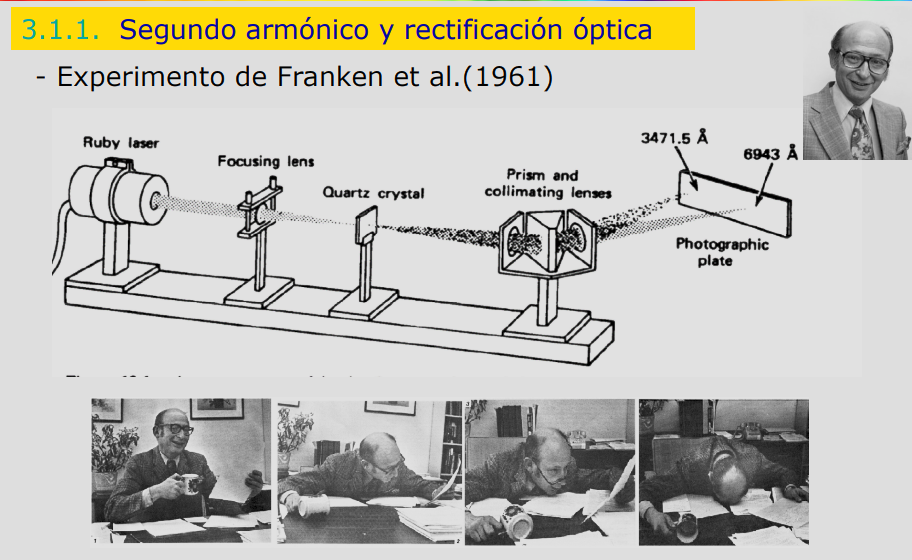
\includegraphics[width=0.7\textwidth]{IMG/segundo.png}
	\end{figure}
	
	\esp
	
	En esta sección, vamos a describir brevemente algunos efectos no lineales que pueden tener lugar cuando una onda e.m. con frecuencia dentro del visible se propaga por un medio con respuesta no lineal. La diferencia fundamental con los efectos descritos en la sección anterior es entonces la frecuencia de modulación del campo, que es mucho más elevada en el caso de ondas luminosas. Igual que en la sección anterior, distinguimos entre efectos de segundo orden y de tercer orden en $P$.
	
	\esp
	
	Dentro de los efectos de segundo orden, describiremos en primer lugar el proceso de generación del segundo armónico y el término de rectificación óptica (que fue el primero en descubrirse). Nos centraremos luego en los procesos de mezcla de tres ondas y sus diferentes aplicaciones.
	
	\esp
	
	Dentro de los efectos de tercer orden, veremos muy brevemente la generación del tercer armónico y algunos efectos y aplicaciones de la mezcla de cuatro ondas.
	
	\esp
	
	\begin{figure}[H]
		\centering
		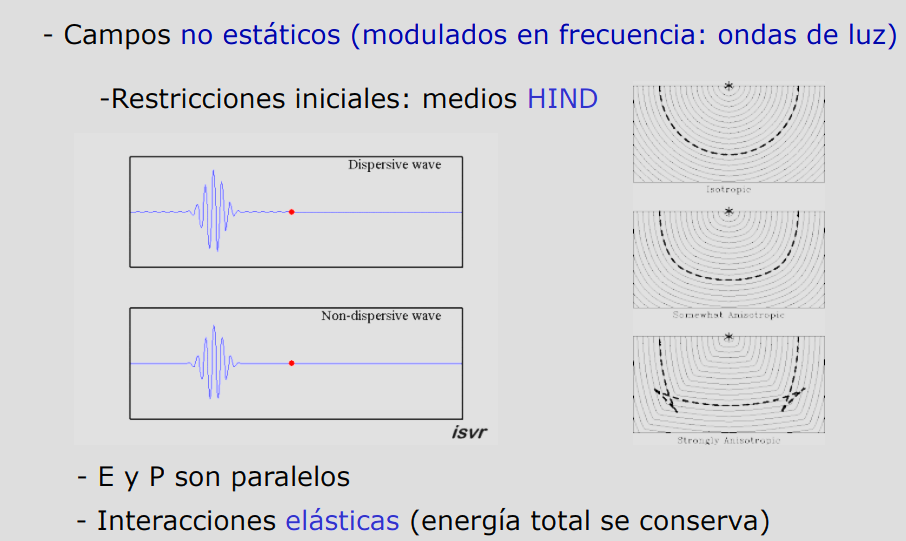
\includegraphics[width=0.7\textwidth]{IMG/segundo2.png}
	\end{figure}
	
	\esp
	
	\begin{figure}[H]
		\centering
		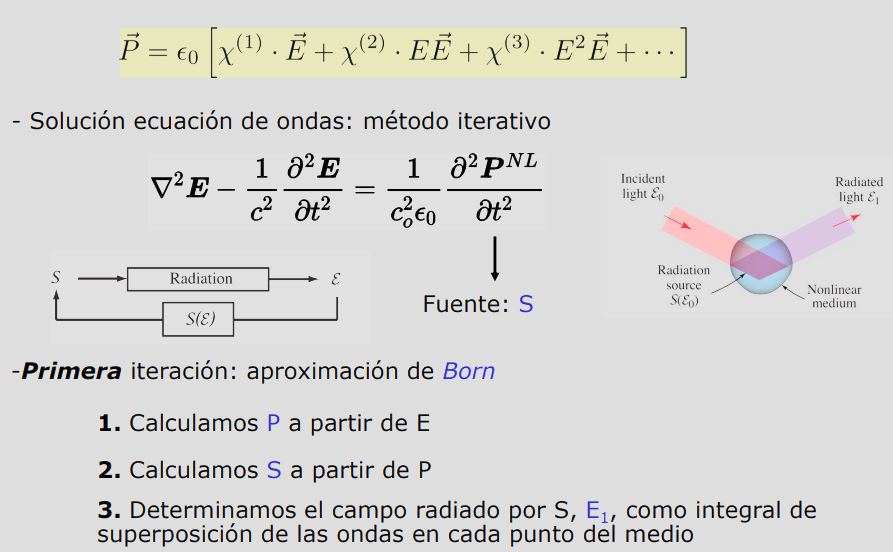
\includegraphics[width=0.7\textwidth]{IMG/segundo3.png}
	\end{figure}
	
	\esp
	
	Es importante tener en cuenta las restricciones que vamos a considerar, para empezar por una situación en la que el tratamiento del fenómeno sea relativamente asequible: consideraremos que los medios no lineales son homogéneos, isótropos y no dispersivos. Esto hace que los vectores $\vec{E}$ y $\vec{P}$ sean paralelos, y por tanto la susceptibilidad eléctrica sea un escalar y no un tensor; además, la relación entre ambos vectores puede ser considerada componente a componente. Una descripción breve de lo que sucede para medios dispersivos o anisótropos puede encontrarse en [1], entre otros textos. También hemos visto en la sección anterior ejemplos de interacciones no lineales con campos estáticos en medios anisótropos. Además, consideraremos también interacciones \textit{paramétricas}, es decir, en las que el intercambio de energía puede producirse entre las diferentes ondas que se propagan en el medio utilizando la no linealidad del propio medio, pero no directamente entre las ondas y el medio. Entonces, la energía total de las ondas se va a conservar (intercambio de tipo elástico). Conforme vayamos avanzando en la descripción de los diferentes tipos de efectos, se irán relajando algunas de estas restricciones (sobre todo la de medios no dispersivos e isótropos).
	
	\esp
	
	Volvemos ahora a la ecuación de ondas descrita en la primera sección, y vamos a ver el tratamiento más simple para obtener una solución de la misma, basado en la aproximación de Born. La idea principal de este método es que la radiación generada por la fuente $S = -\frac{1}{\epsilon_0 c^2} \frac{\partial^2 P^{NL}}{\partial t^2}$ produce a su vez un campo eléctrico, que a su vez produce polarización y por tanto genera a su vez otra fuente $S$, y así sucesivamente. Este proceso sugiere utilizar un sistema iterativo para resolver la ecuación, obteniendo términos sucesivos en varios pasos. El primer paso se conoce como \textit{primera aproximación de Born}. La solución encontrada será una buena aproximación a la solución de la ecuación de ondas cuando la intensidad de la onda incidente no sea muy elevada (siempre hablando en términos de óptica no lineal, es decir, que sea lo bastante elevada para producir efectos no lineales, pero no demasiado perceptibles). Los pasos del método serían, esquemáticamente:
	
	\esp
	
	\begin{itemize}
		\item A partir del campo incidente $E_0$ (recordemos que es una onda y no un campo estático), determinar $P_{NL}$ utilizando los correspondientes coeficientes del medio.
		\item Utilizar $P_{NL}$ para obtener la fuente correspondiente $S(E_0)$, calculando la segunda derivada parcial con respecto al tiempo de $P_{NL}$ que aparece en el término $S$.
		\item Determinar la onda radiada por $S(E_0)$, que puede llamarse $E_1$, como una integral de superposición de las diferentes ondas esféricas generadas en cada punto del medio. Este método constituye una alternativa a la deducción sobre la radiación dipolar en el fenómeno del esparcimiento, que se ha descrito en el tema anterior.
	\end{itemize}
	
	\esp
	
	Un punto importante a tener en cuenta es que el campo inicial, $E_0$, puede estar constituido por una o varias ondas (de diferente frecuencia), con lo cual el campo radiado $E_1$ podrá contener componentes de frecuencia no presentes inicialmente en $E_0$. Como se describió en la introducción, la no linealidad del medio dará lugar a la aparición de nuevas ondas a partir de la incidente, lo que podrá a su vez utilizarse en varias aplicaciones interesantes.
	
	\subsection{Efectos de segundo orden}
	
	Consideramos aquí medios con todas las restricciones señaladas anteriormente (homogéneos, isótropos, no dispersivos ni absorbentes) para los cuales el desarrollo de $P$ en función de $E$ puede truncarse en el segundo término, y por tanto, $P_{NL} = \epsilon_0 \chi^{(2)} E^2$ (medios de segundo orden). Veremos la situación que se produce utilizando la primera aproximación de Born, cuando en el medio inciden una o varias ondas. Dado que estamos en primera aproximación, el campo radiado por esparcimiento elástico $E_1$ tendrá las mismas componentes en frecuencia que $S_\omega$, lo que es equivalente a decir que tendrá las mismas componentes en frecuencia que $P_{NL}$, ya que la operación en derivadas parciales para determinar $S_\omega$ a partir de $P_{NL}$ no afecta al contenido en frecuencias de la señal.
	
	\subsubsection{Generación del segundo armónico y rectificación óptica}
	
	\begin{figure}[H]
		\centering
		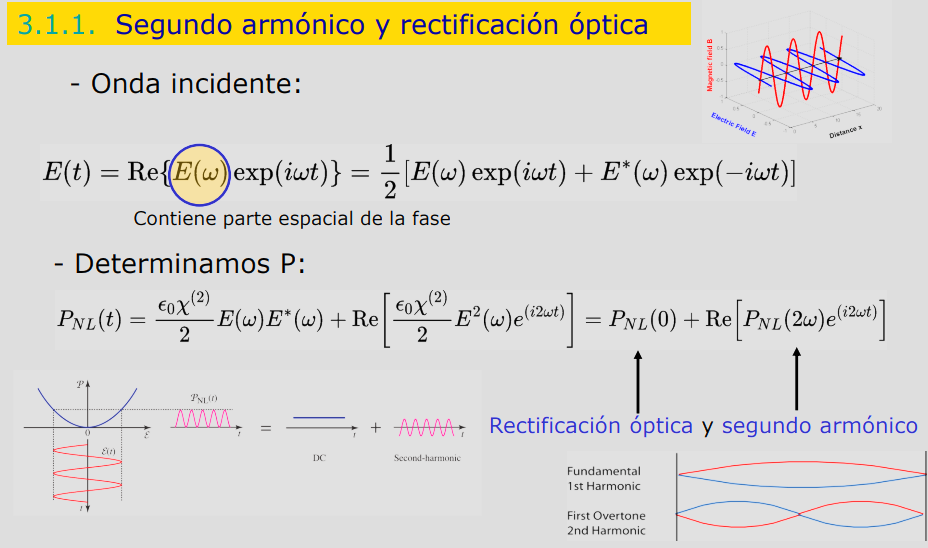
\includegraphics[width=0.7\textwidth]{IMG/segundo4.png}
	\end{figure}
	
	\esp
	
	Suponemos una única onda incidente en un medio no lineal de segundo orden, con frecuencia $\omega$. Podemos expresar entonces el campo incidente como:
	
	\esp
	
	\begin{equation}
		E(t) = \text{Re} \{ E(\omega) \exp(i\omega t) \} = \frac{1}{2} [ E(\omega) \exp(i\omega t) + E^*(\omega) \exp(-i\omega t) ]
	\end{equation}
	
	\esp
	
	El primer término $E(\omega)$ contiene la parte espacial de la fase en la onda inicial. Entonces, utilizamos que $P_{NL} = \epsilon_0 \chi^{(2)} E^2$, y tras operar obtenemos la siguiente expresión para $P_{NL}$:
	
	\esp
	
	\begin{equation}
		P_{NL}(t) = \frac{\epsilon_0 \chi^{(2)}}{2} E(\omega) E^*(\omega) + \text{Re} \left[ \frac{\epsilon_0 \chi^{(2)}}{2} E^2(\omega) e^{i(2\omega t)} \right] = P_{NL}(0) + \text{Re} \left[ P_{NL}(2\omega) e^{i(2\omega t)} \right]
	\end{equation}
	
	\esp
	
	El término $P_{NL}(0)$ se llama \textit{rectificación óptica}, y el segundo término (que indica que $P_{NL}$ contiene una frecuencia que es el doble de la de la onda inicial) dará lugar a la generación del \textit{segundo armónico}, que es en realidad la radiación generada por este término, que tiene la misma distribución en frecuencia que $P_{NL}$. Vamos a describir y discutir algunos detalles de este proceso en primer lugar.
	
	\esp
	
	\begin{figure}[H]
		\centering
		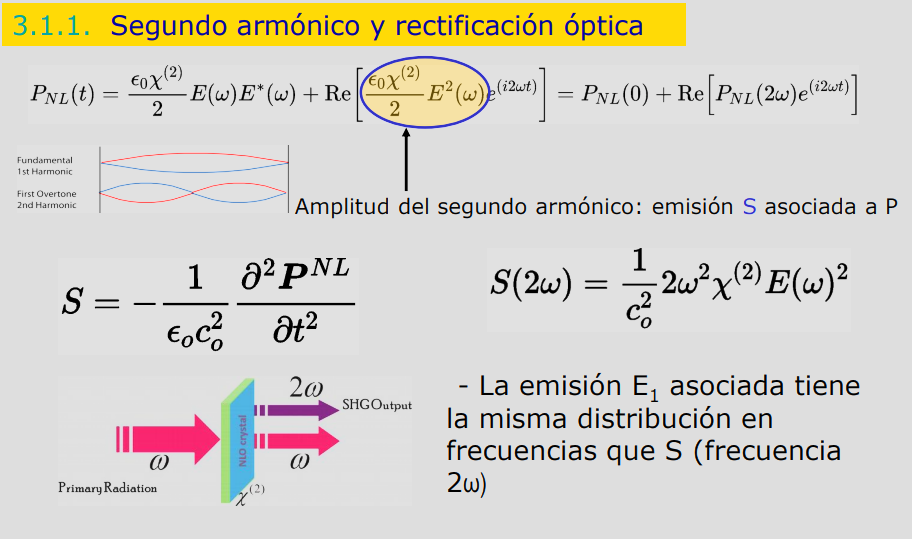
\includegraphics[width=0.7\textwidth]{IMG/segundo5.png}
	\end{figure}
	
	\esp
	
	\textbf{Generación del segundo armónico (Second Harmonic Generation o SHG)}
	El campo $P_{NL}$ generará radiación según su fuente asociada: $S = -\frac{1}{\epsilon_0 c^2} \frac{\partial^2 P_{NL}}{\partial t^2}$, y es inmediato determinar, calculando la segunda derivada parcial, que la amplitud de $S$ será $S(2\omega) = -\frac{1}{2c^2} 2\omega^2 \chi^{(2)} E(\omega)^2$, y la frecuencia de radiación será $2\omega$, como ya se ha mencionado. Entonces, la radiación generada por $S$ contiene términos de frecuencia doble a la de la onda inicial, de ahí su nombre de \textit{segundo armónico}. Vamos a concentrarnos ahora en determinar la intensidad de emisión de este segundo armónico.
	
	\esp
	
	\begin{figure}[H]
		\centering
		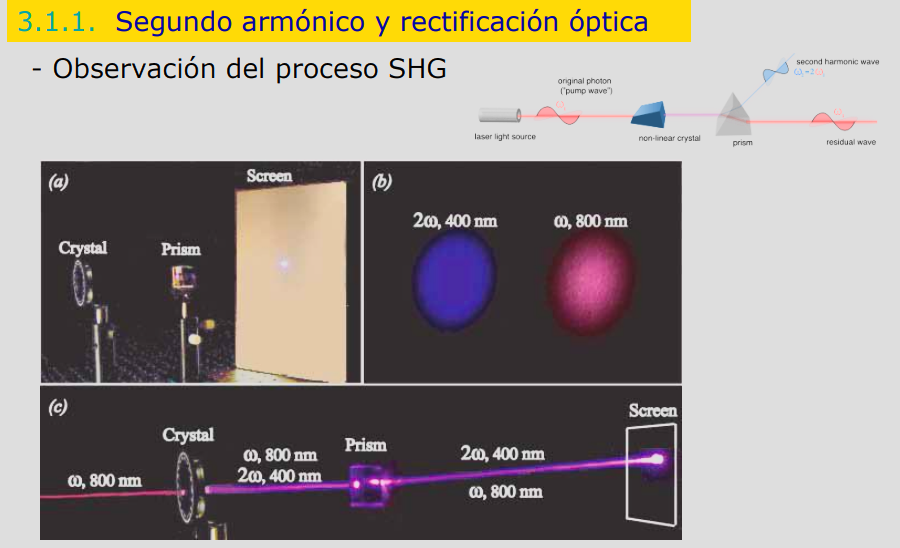
\includegraphics[width=0.7\textwidth]{IMG/segundo6.png}
	\end{figure}
	
	\esp
	
	\begin{figure}[H]
		\centering
		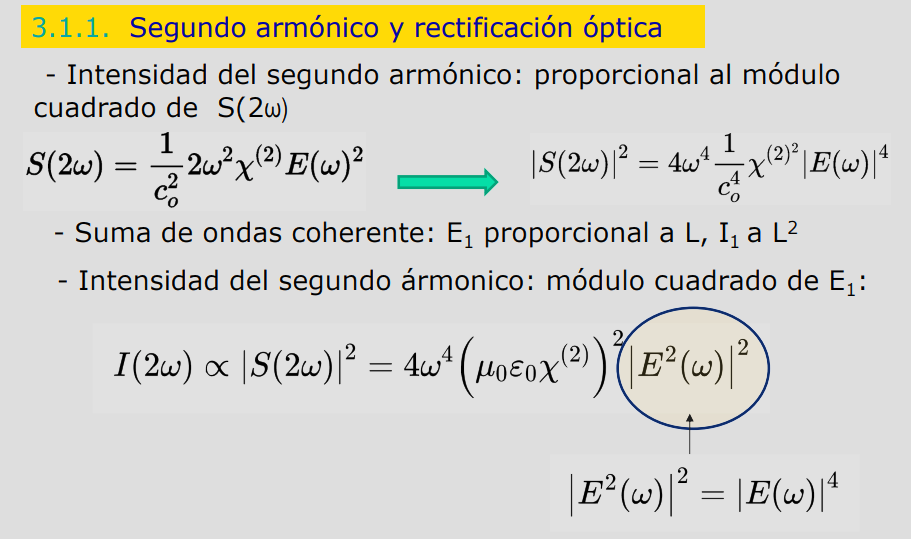
\includegraphics[width=0.7\textwidth]{IMG/segundo7.png}
	\end{figure}
	
	\esp
	
	La intensidad del segundo armónico es entonces proporcional a $|S(2\omega)|^2 = 4\omega^4 \frac{1}{c_0^4} \chi^{(2)^2} |E(\omega)|^4$, por tanto, podemos decir que es proporcional a $I(\omega)^2$, siendo $I(\omega)$ la intensidad de la onda inicial. Además, contiene el cuadrado de un término proporcional a $\chi^{(2)}$. Además, dado que la suma de las diferentes componentes esféricas de la onda se produce de forma coherente, la amplitud resultante es proporcional a la longitud $L$ recorrida del medio. La intensidad queda por tanto proporcional a la cuarta potencia de la frecuencia.
	
	\esp
	
	\begin{figure}[H]
		\centering
		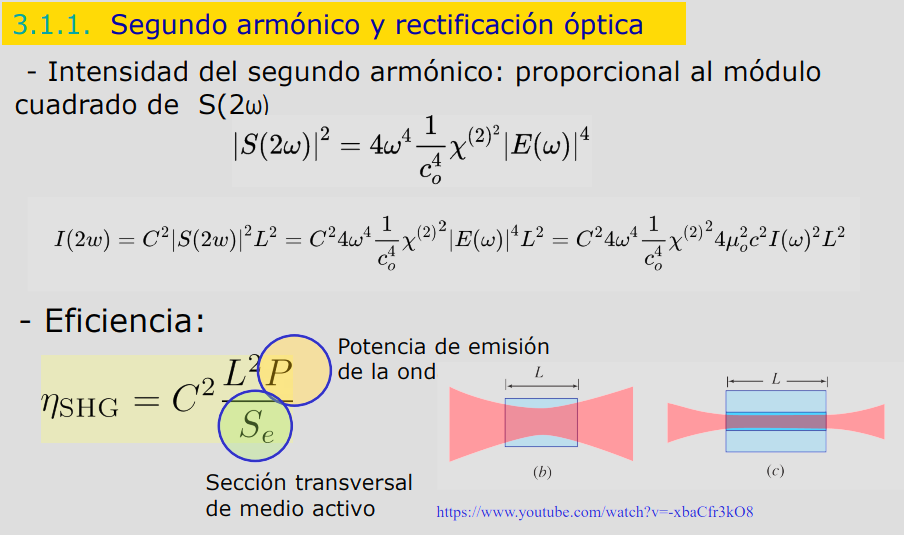
\includegraphics[width=0.7\textwidth]{IMG/segundo8.png}
	\end{figure}
	
	\esp
	
	Un parámetro importante para caracterizar este proceso es la eficiencia $\eta$, definida como la razón entre la intensidad emitida por el segundo armónico y la intensidad de la onda inicial. Si tenemos en cuenta que $I(\omega) = P/S_e$, siendo $S_e$ el área transversal, nos queda:
	
	\esp
	
	\begin{equation}
		\eta_{SHG} = C^2 \frac{L^2 P}{S_e}
	\end{equation}
	
	\esp
	
	En la constante $C$, hemos agrupado los términos dependientes de la frecuencia de la onda y otras constantes. Es interesante también utilizar guías de onda, ya que para estos medios, $S_e$ puede ser relativamente pequeña y $L$ grande. En gran medida, el valor de $\chi^{(2)}$ y la intensidad incidente condicionan la eficiencia. Por ejemplo, para materiales como el KDP se pueden alcanzar eficiencias de centésimas incluso con intensidades de onda inicial del orden de $GW/m^2$. Sin embargo, usando materiales como el betaborato de bario (BBO), se pueden alcanzar hasta el 50\%.
	
	\esp
	
	La generación del segundo armónico tiene como principal aplicación la reducción en la longitud de onda de una fuente: por ejemplo, en un cristal KDP puede tener lugar la conversión de la longitud de onda del láser de Rubí (694 nm) en radiación ultravioleta de 347 nm.
	
	\esp
	
	\begin{figure}[H]
		\centering
		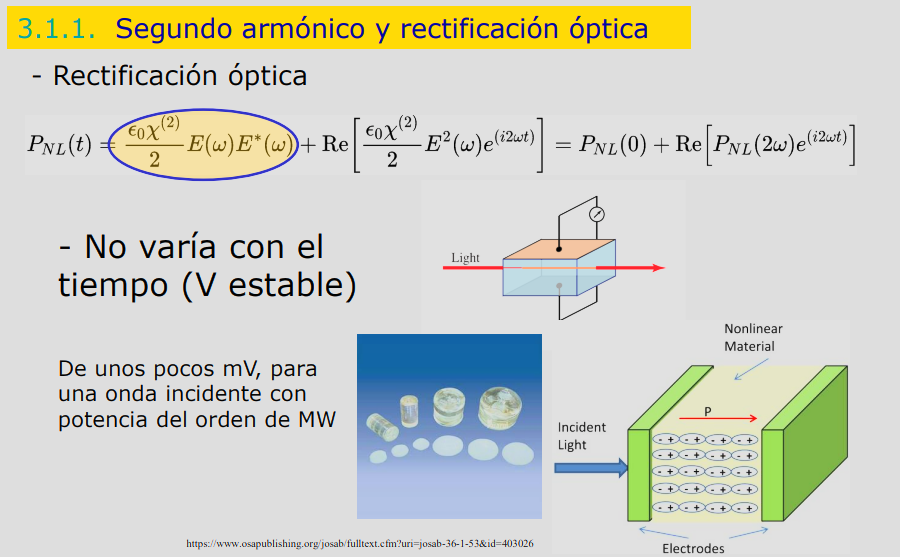
\includegraphics[width=0.7\textwidth]{IMG/segundo9.png}
	\end{figure}
	
	\esp
	
	Vamos a comentar brevemente ahora el primer término (\textit{rectificación óptica} o $P_{NL}(0)$) de la ecuación de la polarización. Esta componente de polarización genera entonces una diferencia de potencial en el medio como consecuencia de la propagación de la onda inicial, de forma análoga a lo que sucede en los dispositivos de conversión de corriente alterna a continua que se llaman \textit{rectificadores}.
	
	\esp
	
	Un aspecto interesante es que, si extendemos el tratamiento para determinar $P_{NL}$ al caso de una combinación de campo estático y onda e.m. de frecuencia $\omega$, puede obtenerse de forma alternativa el tratamiento teórico para el \textit{efecto Pockels} visto en la sección anterior.
	
	\subsection{Mezcla de tres ondas y aplicaciones}
	
	\begin{figure}[H]
		\centering
		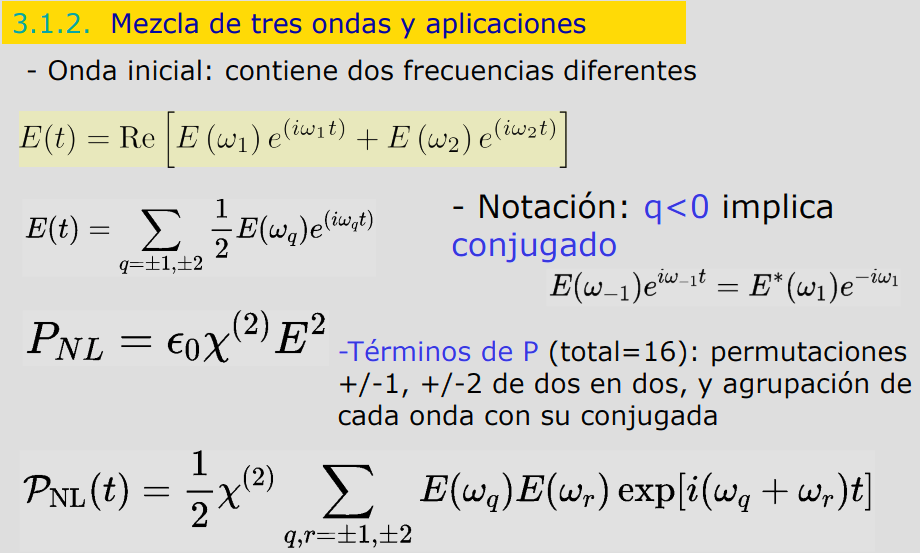
\includegraphics[width=0.7\textwidth]{IMG/tercero.png}
	\end{figure}
	
	\esp
	
	Consideramos ahora qué sucede en un medio no lineal tipo \textit{chi dos}, es decir, no centrosimétrico, cuando en él se propagan dos ondas de frecuencias $\omega_1$ y $\omega_2$. La onda inicial tendría entonces la expresión:
	
	\esp
	
	\begin{equation}
		E(t) = \text{Re} [E (\omega_1) \exp (i\omega_1 t) + E (\omega_2) \exp (i\omega_2 t)]
	\end{equation}
	
	\esp
	
	\begin{figure}[H]
		\centering
		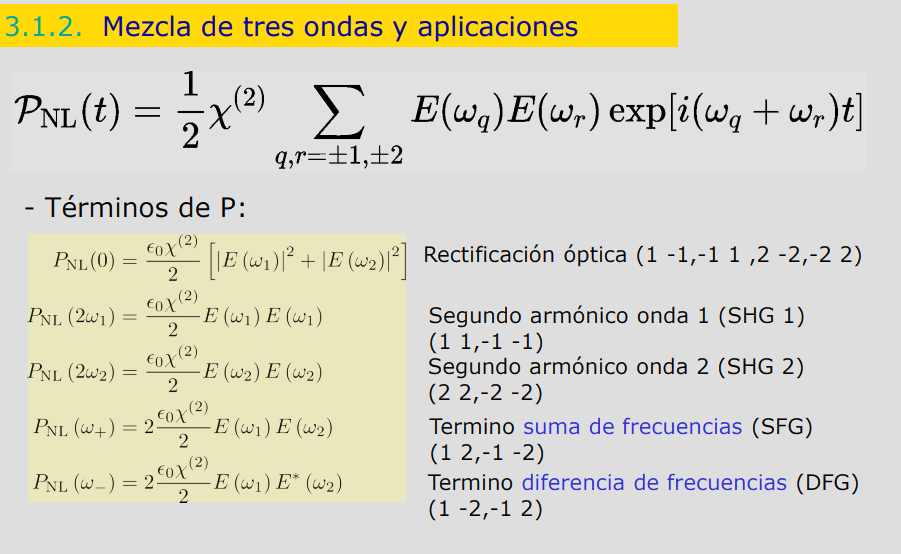
\includegraphics[width=0.7\textwidth]{IMG/tercero2.png}
	\end{figure}
	
	\esp
	
	Siguiendo un desarrollo análogo al caso del segundo armónico, debemos entonces determinar $P_{NL} = \epsilon_0 \chi^{(2)} E^2$. Operando de forma similar y simplificando, nos aparecen entonces cinco términos dentro de $P_{NL}$:
	
	\esp
	
	\begin{align*}
		P_{NL}(0) &= \frac{\epsilon_0 \chi^{(2)}}{2} [|E(\omega_1)|^2 + |E(\omega_2)|^2] \\
		P_{NL}(2\omega_1) &= \frac{\epsilon_0 \chi^{(2)}}{2} E(\omega_1) E(\omega_1) \\
		P_{NL}(2\omega_2) &= \frac{\epsilon_0 \chi^{(2)}}{2} E(\omega_2) E(\omega_2) \\
		P_{NL}(\omega_+) &= 2 \frac{\epsilon_0 \chi^{(2)}}{2} E(\omega_1) E(\omega_2) \\
		P_{NL}(\omega_-) &= 2 \frac{\epsilon_0 \chi^{(2)}}{2} E(\omega_1) E^*(\omega_2)
	\end{align*}
	
	\esp
	
	El primer término sería el de rectificación óptica que ya hemos comentado. Los dos siguientes corresponden a los segundos armónicos de las frecuencias de las ondas iniciales que se propagan por el medio. Al proceso de generación del cuarto término, que tiene una frecuencia suma de las de las ondas iniciales, se le suele llamar \textit{suma de frecuencias}, o más técnicamente \textit{frequency up-conversion}. Al quinto término se le llama entonces \textit{diferencia de frecuencias} o bien \textit{frequency down-conversion} si nos referimos al efecto que da lugar a su origen.
	
	\esp
	
	\begin{figure}[H]
		\centering
		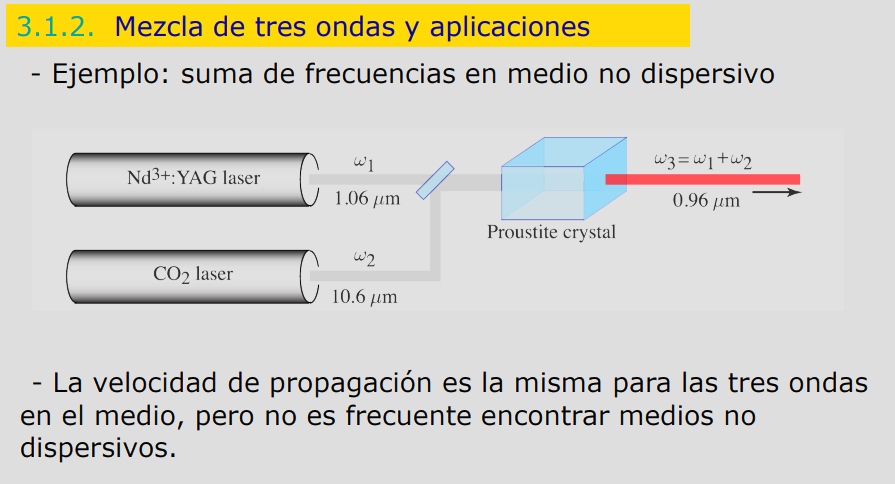
\includegraphics[width=0.7\textwidth]{IMG/tercero3.png}
	\end{figure}
	
	\esp
	
	\begin{figure}[H]
		\centering
		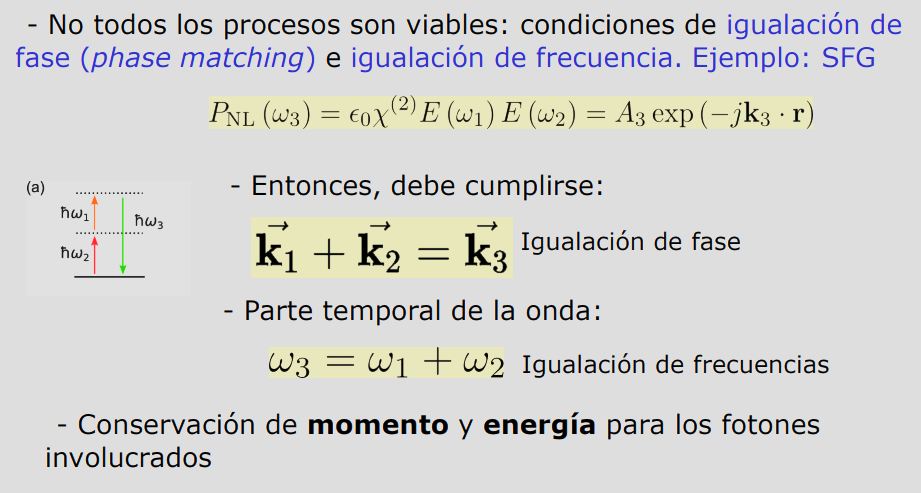
\includegraphics[width=0.7\textwidth]{IMG/tercero4.png}
	\end{figure}
	
	\esp
	
	Entonces, el efecto del medio no lineal es mezclar las frecuencias iniciales y producir una tercera onda de diferente frecuencia (suma o diferencia de las dos que se mezclan). Veremos a continuación cómo puede regularse la amplificación de los diferentes términos para que obtengamos al final sólo una tercera onda de forma efectiva a la salida del medio, como se muestra en la figura para un caso concreto. Notad que, si consideramos un medio no dispersivo, se cumple la relación de las inversas de las longitudes de onda, de modo que $\frac{1}{\lambda_3} = \frac{1}{\lambda_1} + \frac{1}{\lambda_2}$.
	
	\esp
	
	\textbf{Condiciones de igualación de fase (\textit{Phase matching}) y frecuencia}
	Según hemos visto, la amplitud compleja del término de polarización correspondiente a la suma de ondas sería la siguiente:
	
	\esp
	
	\begin{equation}
		P_{NL} (\omega_3) = \epsilon_0 \chi^{(2)} E (\omega_1) E (\omega_2) = \epsilon_0 \chi^{(2)} A_1 A_2 \exp (-j \mathbf{k}_3 \cdot \mathbf{r})
	\end{equation}
	
	\esp
	
	Por tanto, se deduce que se cumple la siguiente condición para los números de onda de las tres ondas:
	
	\esp
	
	\begin{equation}
		\mathbf{k}_1 + \mathbf{k}_2 = \mathbf{k}_3
	\end{equation}
	
	\esp
	
	Y, por supuesto, también se cumple la condición de que $\omega_3 = \omega_1 + \omega_2$. La onda generada por la interacción de las dos ondas iniciales con el medio no lineal debe cumplir entonces la condición sobre los números de onda (condición de \textit{Phase matching} o igualación de fase) además de la condición sobre las frecuencias. Esta condición es necesaria para que las tres ondas puedan interactuar mutuamente durante un cierto período de tiempo, de forma estable.
	
	\esp
	
	\begin{figure}[H]
		\centering
		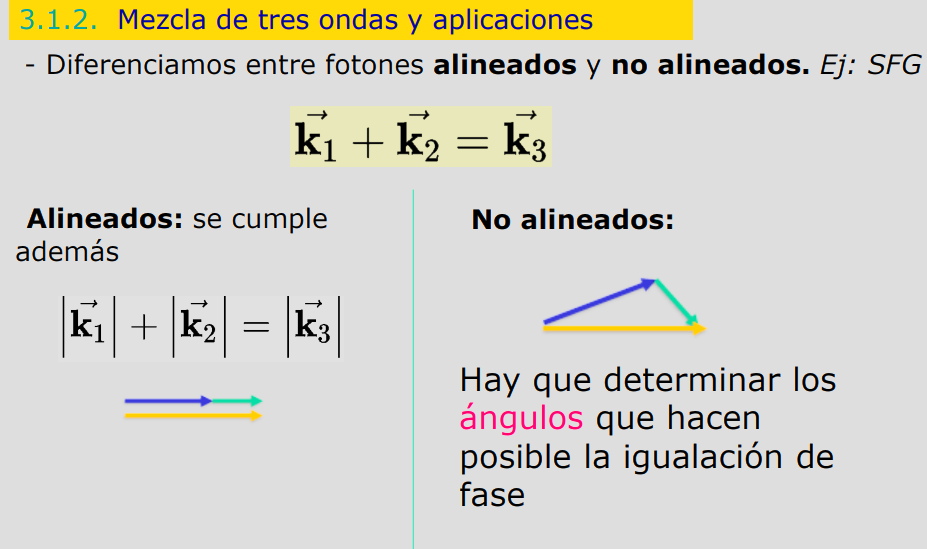
\includegraphics[width=0.7\textwidth]{IMG/tercero5.png}
	\end{figure}
	
	\esp
	
	De forma alternativa y más simple, se puede ver el proceso no lineal como un proceso a nivel de fotones, en el que dos fotones de frecuencias $\omega_1$ y $\omega_2$ son destruidos y se genera un nuevo fotón de frecuencia $\omega_3$. Dado que debe conservarse la energía en el proceso con las restricciones que nos hemos marcado, se cumple la condición de suma de frecuencias. Y la condición de igualación de fase se derivaría de la conservación del momento para los tres fotones involucrados.
	
	\esp
	
	Como hemos dicho, si nos aseguramos de que se cumplen ambas condiciones, se da lugar a un proceso generalizado de \textit{mezcla de tres ondas} que puede presentar muchas variantes, como veremos a continuación. Si las otras ondas generadas en el medio no se sostienen porque no cumplen las condiciones de igualación de fase, entonces tenemos posibles interacciones entre la onda de frecuencia $\omega_3$ y la onda de frecuencia $\omega_2$, generándose por ejemplo una onda en un proceso de resta de frecuencias, que tendría una frecuencia $\omega_1$. Igualmente, la onda de frecuencia $\omega_3$ puede interactuar con la onda de frecuencia $\omega_1$ generando una onda de frecuencia $\omega_2$ por diferencia de frecuencias. Así, las tres ondas pueden ir interactuando y sosteniéndose mutuamente en el medio no lineal. Este proceso se llama entonces \textit{mezcla de tres ondas}.
	
	\esp
	
	Las variantes de este proceso paramétrico de mezcla de tres ondas dependen de qué ondas funcionen como entrada y cuáles se seleccionen a la salida del medio no lineal. Algunos de estos procesos los vamos a describir específicamente a continuación, y se muestran esquemáticamente en la figura 5.
	
	\esp
	
	\begin{itemize}
		
		\begin{figure}[H]
			\centering
			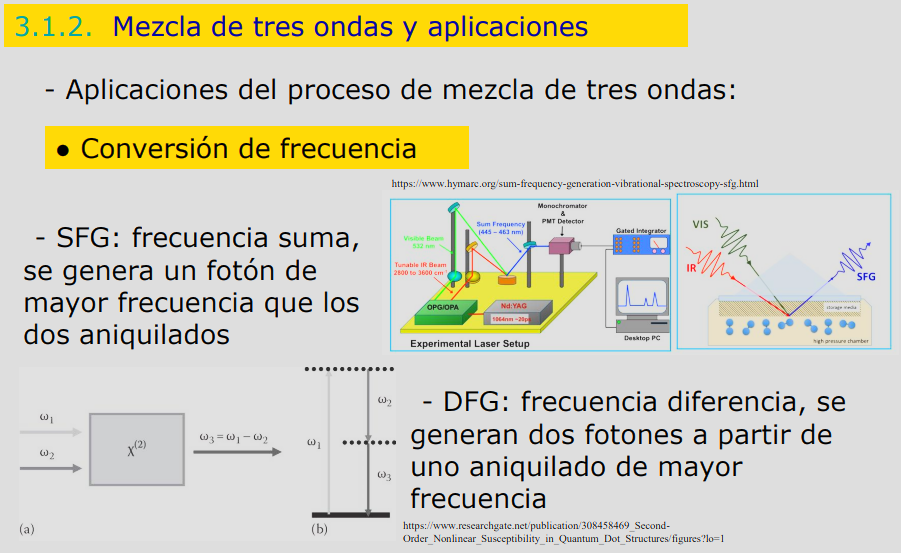
\includegraphics[width=0.7\textwidth]{IMG/tercero6.png}
		\end{figure}
		
		\esp
		
		\item \textbf{Conversión óptica de frecuencia.} Incluye dos procesos: la generación de la frecuencia suma (SFG), que ya hemos descrito antes, en el que las ondas de frecuencia $\omega_1$ y $\omega_2$ entran al material, y se genera una tercera onda de frecuencia $\omega_3 = \omega_1 + \omega_2$. El proceso complementario a éste se llama generación de la frecuencia resta o \textit{DFG}. En el DFG las ondas de frecuencia $\omega_3$ y $\omega_1$ interactúan para generar una onda de frecuencia $\omega_2$. Si la onda 1 y la onda 2 tienen la misma frecuencia, puede verse el proceso SHG como una versión particular de un proceso SFG, que se llama \textit{degenerada}.
		
		\esp
		
		\begin{figure}[H]
			\centering
			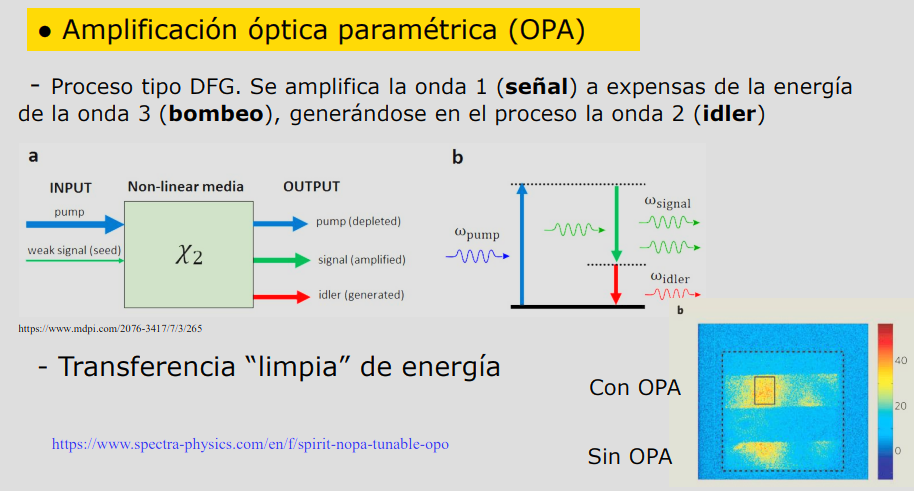
\includegraphics[width=0.7\textwidth]{IMG/tercero7.png}
		\end{figure}
		
		\esp
		
		\item \textbf{Amplificación óptica paramétrica (OPA).} Es un proceso tipo DFG en el que la onda de frecuencia $\omega_3$ (bombeo) interactúa con la onda de frecuencia $\omega_1$ (señal), de forma que ésta se amplifica, creándose también en el proceso otra onda de frecuencia $\omega_2$ (\textit{idler} o inerte). Los OPA se suelen usar para permitir la detección de ondas de señal débil para las cuales no es posible utilizar detectores de alta sensibilidad.
		
		\esp
		
		\begin{figure}[H]
			\centering
			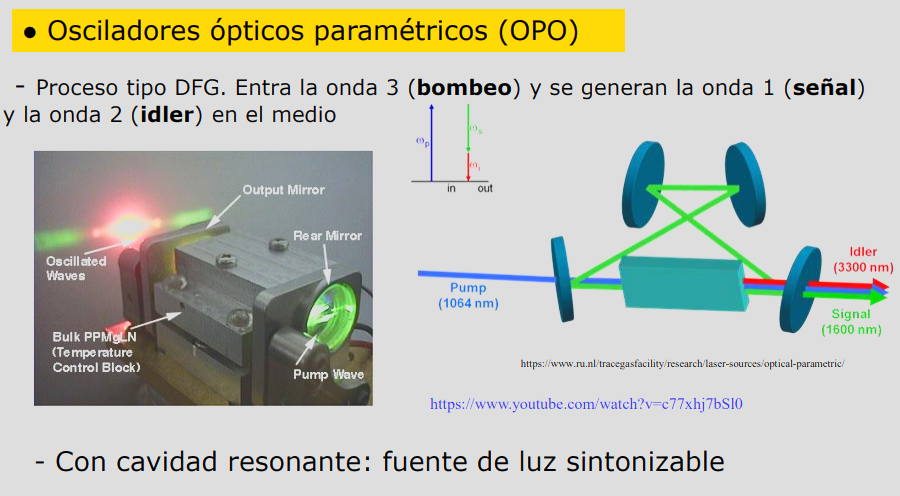
\includegraphics[width=0.7\textwidth]{IMG/tercero8.png}
		\end{figure}
		
		\esp
		
		\item \textbf{Optical Parametric Oscillation (OPO).} Es una variante del proceso anterior en la cual al medio se suministra sólo la onda \textit{de bombeo}, y se genera las ondas \textit{señal} e \textit{idler} en el propio medio. Se pueden utilizar entonces como fuentes de luz sintonizables, puesto que la frecuencia generada puede variar en función de algunos parámetros del medio, como la temperatura.
		
		\esp
		
		\begin{figure}[H]
			\centering
			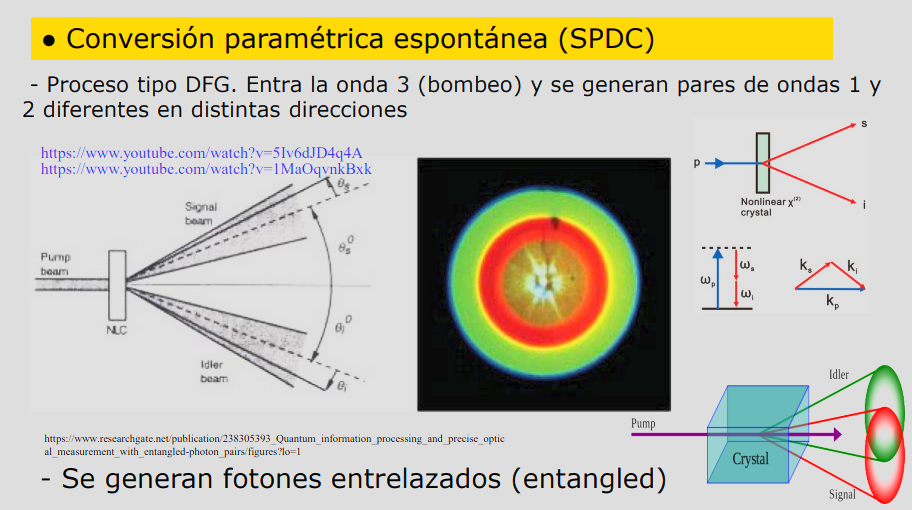
\includegraphics[width=0.7\textwidth]{IMG/tercero9.png}
		\end{figure}
		
		\esp
		
		\item \textbf{Conversión paramétrica espontánea (SPD).} En este proceso (de nuevo, una variante de DFG), se suministra al medio la onda 3 (bombeo), y se generan varios posibles pares de frecuencias $\omega_1$ y $\omega_2$, que cumplen la condición de igualación de fase y frecuencia. La característica más destacable del proceso es que las dos ondas generadas se propagan en direcciones distintas, y están entrelazadas cuánticamente. El resultado es un cono de ondas multiespectral.
	\end{itemize}
	
	\esp
	
	\textbf{Igualación de fase y curvas de sintonizado} Vamos a ver por último en este apartado algunos casos particulares de condiciones de igualación de fase, y cómo pueden aprovecharse las características del medio para asegurar que se cumplan las condiciones de igualación de fase, o bien cómo estas pueden relajarse hasta cierto punto.
	
	\esp
	
	\begin{figure}[H]
		\centering
		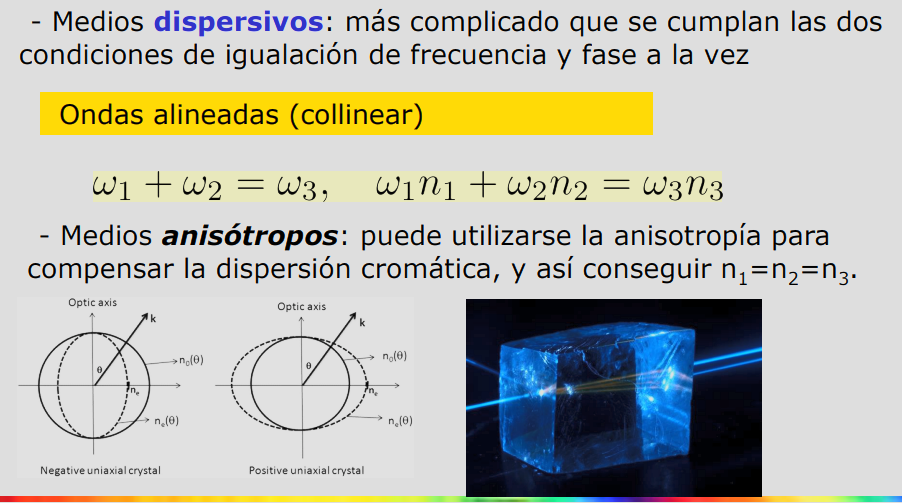
\includegraphics[width=0.7\textwidth]{IMG/tercero10.png}
	\end{figure}
	
	\esp
	
	\textbf{Ondas alineadas en dirección de propagación} En el caso de mezcla de tres ondas alineadas, es decir, que se propagan en la misma dirección, entonces las condiciones de igualación de frecuencia y fase quedarían de la siguiente forma:
	
	\esp
	
	\begin{equation}
		\omega_1 + \omega_2 = \omega_3, \quad \omega_1 n_1 + \omega_2 n_2 = \omega_3 n_3
	\end{equation}
	
	\esp
	
	Esto se deduce utilizando el hecho de que los vectores $\mathbf{k}_1$, $\mathbf{k}_2$ y $\mathbf{k}_3$ serían paralelos, y la relación entre $k$ y $n$ a través de la frecuencia y la velocidad de la luz en el vacío.
	
	\esp
	
	Debido a que los medios son normalmente dispersivos, las ondas viajan con diferente índice de refracción, y por tanto no suelen poder cumplirse las dos condiciones de igualación de frecuencia y fase a la vez. Sin embargo, si el medio es anisótropo, puede utilizarse esto para compensar la dispersión cromática, y así hacer posible que se cumplan las dos condiciones a la vez, y por tanto que se den los procesos no lineales. Empezamos ya a relajar las restricciones impuestas al principio de la sección.
	
	\esp
	
	\begin{figure}[H]
		\centering
		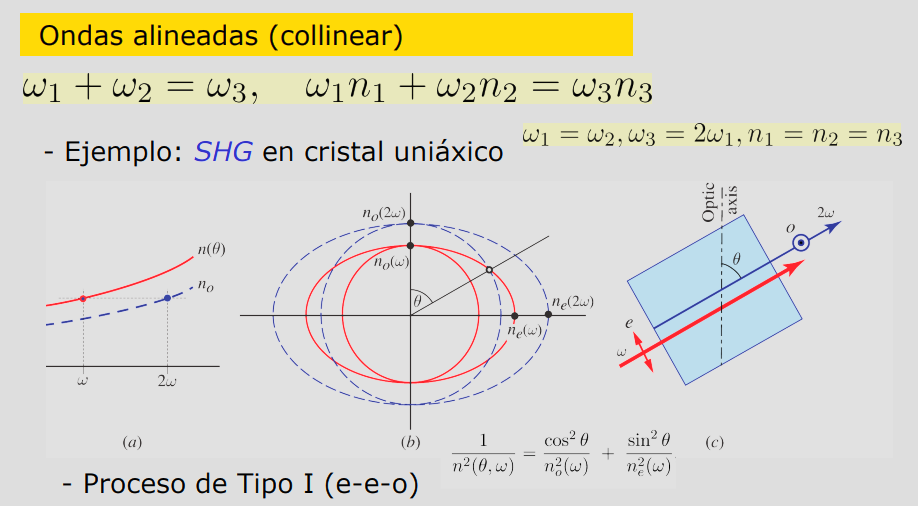
\includegraphics[width=0.7\textwidth]{IMG/tercero11.png}
	\end{figure}
	
	\esp
	
	Veamos un ejemplo referido a la generación del segundo armónico (SHG) en un cristal uniáxico de índices propios $n_o$ y $n_e$. Vamos a suponer que las dos ondas incidentes en el medio tienen la misma frecuencia ($\omega_1 = \omega_2$, como corresponde al proceso de SHG) y la misma dirección de vibración, con lo cual tienen también el mismo índice de refracción ($n_1 = n_2$). La frecuencia de la onda 3 es entonces la del segundo armónico ($\omega_3 = 2\omega_1$). Por tanto, la condición de igualación de fase impone que también se cumpla que $n_3 = n_1$. O sea, que el segundo armónico viaje a la misma velocidad en el medio que las ondas 1 y 2 (o que la onda inicial a secas). Debido a la dispersión del medio, esto no va a producirse, salvo que podamos jugar con la birrefringencia del mismo y la polarización de la onda 3 para que dicha onda se propague a la misma velocidad que las ondas 1 y 2, como se ilustra en la figura 6. Puede encontrarse la solución adecuada para el ángulo de incidencia utilizando la ecuación de cálculo de las velocidades que se vio en Óptica I para la propagación de las ondas, e imponiendo que $n(\theta, \omega) = n_o(2\omega)$.
	
	\esp
	
	El proceso ilustrado en la figura decimos que es de \textit{Tipo I} porque las dos ondas que se suman tienen la misma dirección de vibración (estado de polarización). En concreto, se trata de un proceso \textit{e-e-o}, ordenando las etiquetas de estado de polarización ($e$ indica extraordinario, $o$ ordinario) de menor a mayor frecuencia. En algunos medios, la solución encontrada para los procesos de \textit{upconversion} o \textit{downconversion} requiere que las ondas de menor frecuencia tengan diferentes direcciones de vibración. En ese caso, hablamos de procesos \textit{Tipo II}. Un ejemplo de procesos de este tipo sería \textit{o-e-o}.
	
	\esp
	
	Como vemos, dado que las velocidades serán iguales sólo para ciertas direcciones de propagación dentro del medio (las que permitan que la onda ordinaria del segundo armónico viaje a igual velocidad que la onda extraordinaria de la señal inicial), si representamos la intensidad a la salida del medio del segundo armónico en función del ángulo de incidencia, se irán obteniendo picos y valles dependiendo de si se cumple la condición de igualación de fase o no para esa dirección de incidencia. Por ejemplo, para un cristal de KDP y una onda incidente de 694 nm, $n_e = 1,534$ y $n_o = 1,490$, así que se puede encontrar un ángulo $\theta = 52^\circ$ que cumpla la condición de igualación de fase con un proceso tipo I \textit{o-o-e}. Lo que suele hacerse es cortar el cristal y orientarlo de forma que se produzca la dirección de propagación en el interior del mismo que buscamos.
	
	\esp
	
	Para muchas aplicaciones prácticas, por ejemplo un OPO, puede representarse la longitud de onda (determinada a partir del índice de refracción, obtenido con la ecuación de Sellmeier que se mencionó en el tema anterior y la superficie de las velocidades) para las ondas 1 y 2, en función del ángulo de refracción en el cristal, y determinar así si existe algún ángulo en el que las dos curvas se corten y que permita por tanto que el proceso sea sostenible. A estas curvas se llama \textit{Curvas de sintonizado} o \textit{Phase tuning curves}.
	
	\esp
	
	\begin{figure}[H]
		\centering
		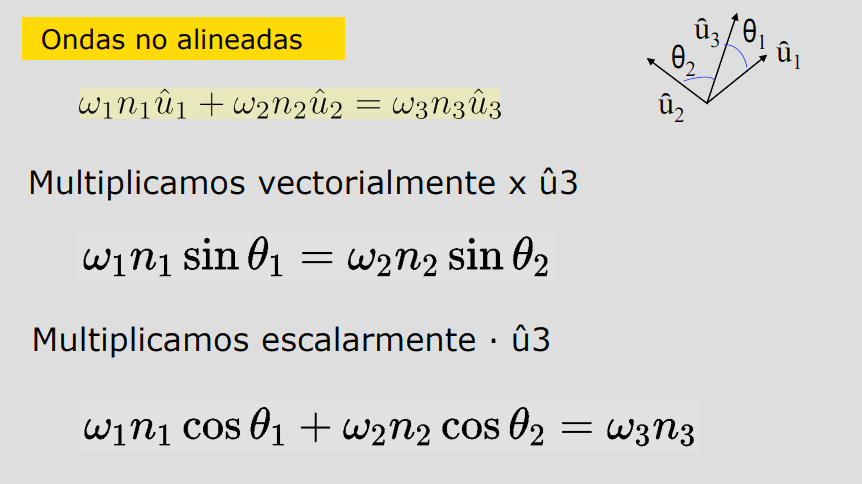
\includegraphics[width=0.7\textwidth]{IMG/tercero12.png}
	\end{figure}
	
	\esp
	
	\textbf{Ondas no alineadas (con diferente dirección de propagación)} En este caso, tenemos una condición de igualación de fase en la que intervienen los vectores según las tres direcciones de propagación:
	
	\esp
	
	\begin{equation}
		\omega_1 n_1 \hat{u}_1 + \omega_2 n_2 \hat{u}_2 = \omega_3 n_3 \hat{u}_3
	\end{equation}
	
	\esp
	
	Si multiplicamos esta ecuación escalarmente por el vector unitario perpendicular a $\hat{u}_3$, y luego por el propio vector $\hat{u}_3$, obtenemos dos ecuaciones en función de los ángulos que formen las direcciones $\hat{u}_1$ y $\hat{u}_2$ con $\hat{u}_3$:
	
	\esp
	
	\begin{equation}
		\omega_1 n_1 \operatorname{sen} \theta_1 = \omega_2 n_2 \operatorname{sen} \theta_2, \quad \omega_1 n_1 \cos \theta_1 + \omega_2 n_2 \cos \theta_2 = \omega_3 n_3
	\end{equation}
	
	\esp
	
	Recordemos que los índices de refracción van a depender de las direcciones de propagación y de las direcciones de vibración de las tres ondas, en el caso de medios anisótropos. Por tanto, si queremos que funcione el proceso no lineal en esta situación, deberemos seleccionar tanto las direcciones de propagación como las direcciones de vibración de las ondas, para que se pueda cumplir la condición de igualación de fase además de la de igualación de frecuencia.
	
	\esp
	
	\begin{figure}[H]
		\centering
		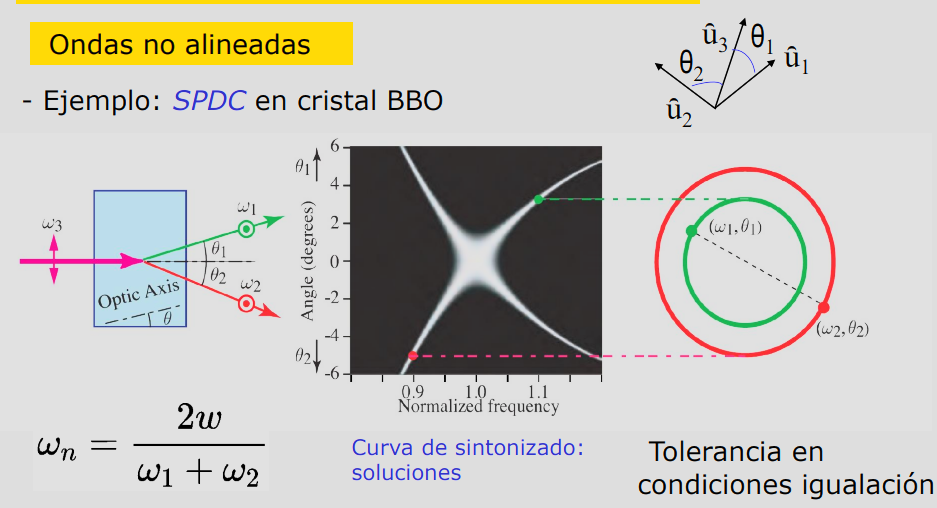
\includegraphics[width=0.7\textwidth]{IMG/tercero13.png}
	\end{figure}
	
	\esp
	
	Veamos un ejemplo del proceso de \textit{SPDC: conversión paramétrica espontánea hacia abajo} en un cristal BBO (borato de bario beta). La onda de bombeo es de 351,5 nm, y el proceso es tipo \textit{o-o-e}, es decir, que las polarizaciones de las ondas 1 y 2 (señal e \textit{idler}) son normales a la sección principal del cristal (que coincide en este ejemplo con el plano de incidencia), y la polarización de la onda de bombeo está contenida en la sección principal, como se muestra en la figura. En este ejemplo, el ángulo $\theta$ que forma el eje óptico con la dirección de propagación en el interior del cristal es $33,53^\circ$, y en el medio se van a generar las ondas 1 y 2 con frecuencias y direcciones de propagación que puedan satisfacer las condiciones de igualación de fase y frecuencia. Considerando las ecuaciones de dependencia del índice de refracción con la frecuencia, la ecuación de cálculo de las velocidades en el medio y las condiciones de igualación de fase, una fracción de las posibles soluciones está representada en la parte central de la figura 7. En el eje horizontal de esta figura central se representa $\frac{2\omega}{\omega_3}$, o sea, la frecuencia normalizada con respecto al caso \textit{degenerado} en el que $\omega_1 = \omega_2 = \frac{\omega_3}{2}$.
	
	\esp
	
	Lo que hacemos para encontrar un par de frecuencias que puedan dar lugar al proceso es entonces lo siguiente: supongamos que fijamos la frecuencia $\omega_1 = 1,1 \frac{\omega_3}{2}$. Entonces, el brazo superior de la curva de sintonizado nos daría un ángulo $\theta_1$ de $3^\circ$ aproximadamente. Dado que tiene que cumplirse la condición de igualación de frecuencias, entonces ya sabemos que nuestra frecuencia $\omega_1$ generará una onda idler de frecuencia $\omega_2 = 0,9 \frac{\omega_3}{2}$. Buscamos dicha frecuencia en la curva siguiendo el brazo correspondiente en la parte inferior de la figura, y llegamos al ángulo $\theta_2$, que sería de $-5^\circ$ aproximadamente. Esta es sólo una de las múltiples posibles soluciones, pero podríamos escoger la solución que queramos insertando los filtros necesarios a la salida del cristal, o alimentando el medio con la frecuencia de la señal que queramos obtener a la salida. Como vemos ilustrado en la parte derecha de la figura, habría simetría circular y tendríamos un cono con sección circular a la salida del medio, pero cada punto de este anillo de emisión de la señal estaría emparejado sólo con un punto diametralmente opuesto del anillo correspondiente a la frecuencia de la onda \textit{idler}.
	
	\esp
	
	Hay una cierta tolerancia para las condiciones de igualación de fase y frecuencia, a expensas de reducir la eficiencia de los procesos no lineales. Por ejemplo, en la figura 7 vemos que hay una cierta anchura en las curvas de sintonizado, lo cual muestra que para este proceso, en especial si la frecuencia está próxima al caso degenerado, se podrían producir ondas viables en el medio que no cumpliesen exactamente la condición de igualación de frecuencia. Como puede verse desarrollado en [1], cap. 22, la tolerancia va a depender de parámetros del medio como son la longitud de medio activo $L$, de forma que la eficiencia del proceso es casi nula cuando hay una diferencia entre las fases $k_3 - (k_1 + k_2) = \frac{2\pi}{L}$. Considerando esto de otra forma, podríamos fijar un determinado intervalo $\Delta \vec{k}$, y calcular la longitud de medio activo para la cual el proceso no lineal ya dejaría de ser viable, también conocida como \textit{distancia de coherencia}. Es importante no confundir este parámetro con la longitud de coherencia relacionada con la coherencia temporal de las fuentes de luz, que vimos en Óptica I.
	
	\esp
	
	En la siguiente sección, vamos a describir algunos aspectos relevantes de los procesos no lineales de tercer orden.
	
	\subsection{Efectos de tercer orden}
	
	\begin{figure}[H]
		\centering
		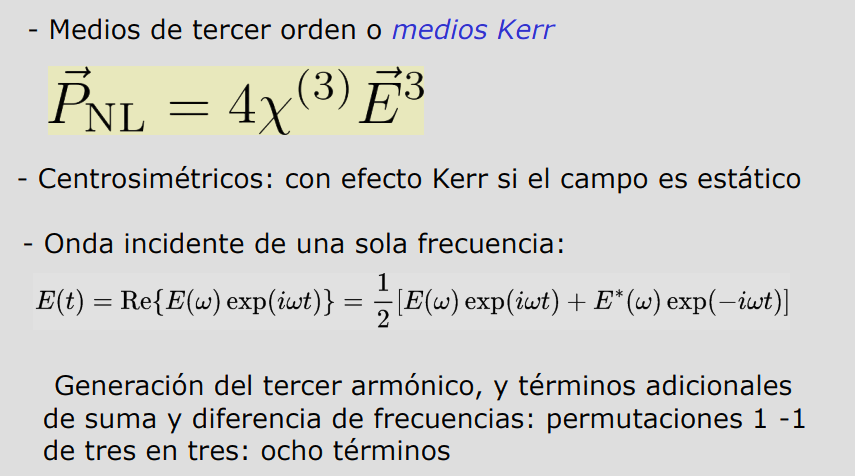
\includegraphics[width=0.7\textwidth]{IMG/tercero14.png}
	\end{figure}
	
	\esp
	
	Como ya hemos discutido al tratar el efecto Kerr, en medios centrosimétricos, los términos no lineales de segundo orden en la expresión para $\vec{P}$ en función de $\vec{E}$ no pueden darse. Entonces, el primer término no lineal que aparece es un término de tercer orden. Consideramos, por comodidad, la permeabilidad $\epsilon_0$ incluida dentro del coeficiente $\chi^{(3)}$.
	
	\esp
	
	\begin{equation}
		\vec{P}_{NL} = 4\chi^{(3)} \vec{E}^3
	\end{equation}
	
	\esp
	
	Estos medios se llaman entonces \textit{medios de tercer orden} o \textit{medios Kerr}. Estos medios presentan el efecto Kerr descrito en secciones anteriores, cuando están sometidos a campos estáticos.
	
	\esp
	
	En el caso de propagarse ondas de luz muy intensas por ellos, se generarán terceros armónicos y términos de suma y diferencia de tres frecuencias.
	
	\esp
	
	\subsubsection{Generación del tercer armónico}
	
	Haciendo un desarrollo análogo al visto para la generación del segundo armónico (SHG), considerando un campo incidente de la siguiente forma:
	
	\esp
	
	\begin{equation}
		E(t) = \text{Re}\{E(\omega) \exp(i\omega t)\} = \frac{1}{2} [E(\omega) \exp(i\omega t) + E^*(\omega) \exp(-i\omega t)]
	\end{equation}
	
	\esp
	
	\begin{figure}[H]
		\centering
		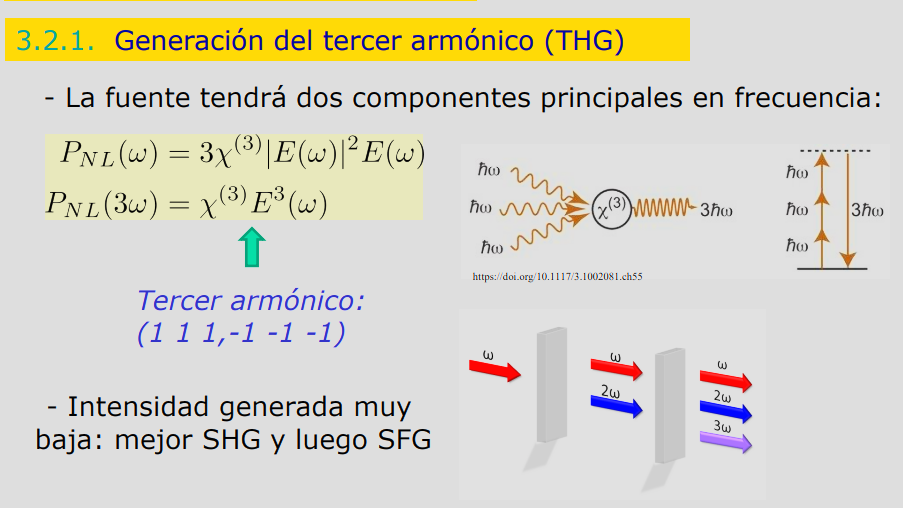
\includegraphics[width=0.7\textwidth]{IMG/tercero15.png}
	\end{figure}
	
	\esp
	
	\noindent Al elevar al cubo obtenemos dos componentes de frecuencia principales:
	
	\esp
	
	\begin{align*}
		P_{NL}(\omega) &= 3\chi^{(3)} |E(\omega)|^2 E(\omega) \\
		P_{NL}(3\omega) &= \chi^{(3)} E^3(\omega)
	\end{align*}
	
	\esp
	
	La segunda componente corresponde al \textit{tercer armónico}. Sin embargo, debido al valor de $\chi^{(3)}$, la intensidad generada suele ser muy reducida, con lo que la eficiencia del proceso es baja. De hecho, suele abordarse la generación del tercer armónico como un proceso de suma de frecuencias a partir de otro proceso de SHG.
	
	\subsubsection{Efecto Kerr óptico}

	\begin{figure}[H]
		\centering
		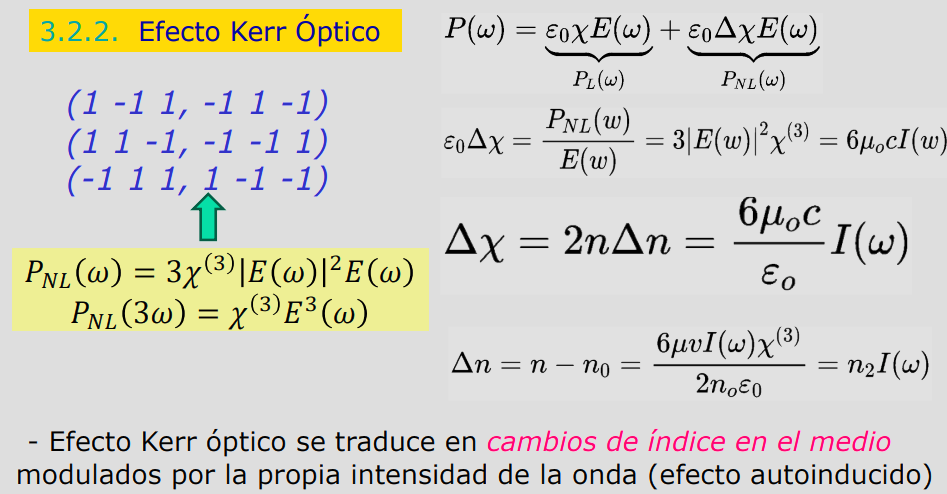
\includegraphics[width=0.7\textwidth]{IMG/tercero16.png}
	\end{figure}
	
	\esp
	
	La no linealidad de tercer orden en $\vec{P}$ se traduce también en un cambio de susceptibilidad eléctrica para el medio, expresado a través del primer término en $P_{NL}$, de forma que:
	
	\esp
	
	\begin{equation}
		\epsilon_0 \Delta\chi = \frac{P_{NL}(\omega)}{E(\omega)} = 3\chi^{(3)} |E(\omega)|^2
	\end{equation}
	
	\esp
	
	Así, la variación en susceptibilidad eléctrica resulta proporcional a la intensidad de la onda incidente, y (dado que los incrementos son pequeños), puede aproximarse el cambio en el índice de refracción de forma que también resulta proporcional a dicha intensidad. Así, el índice de refracción quedaría como:
	
	\esp
	
	\begin{equation}
		n = n_0 + n_2 I
	\end{equation}
	
	\esp
	
	\noindent siendo $n_2$ proporcional a $\chi^{(3)}$.
	
	\esp
	
	Es una expresión similar a la vista en las secciones anteriores para el efecto Kerr eléctrico (con campos estáticos), y refleja un fenómeno de refracción \textit{no lineal} para el cual la velocidad de fase depende directamente de la intensidad de la onda incidente. El orden de magnitud de $n_2$ va desde $10^{-16}$ para algunos cristales, hasta $0,01$ en algunos semiconductores.
	
	\esp
	
	Después de esta descripción de dos fenómenos básicos derivados de los dos términos principales de $P_{NL}$, vamos a tratar algunas aplicaciones derivadas de procesos algo más elaborados en las siguientes subsecciones.
	
	\subsubsection{Automodulación de fase (SPM)}
	
	\begin{figure}[H]
		\centering
		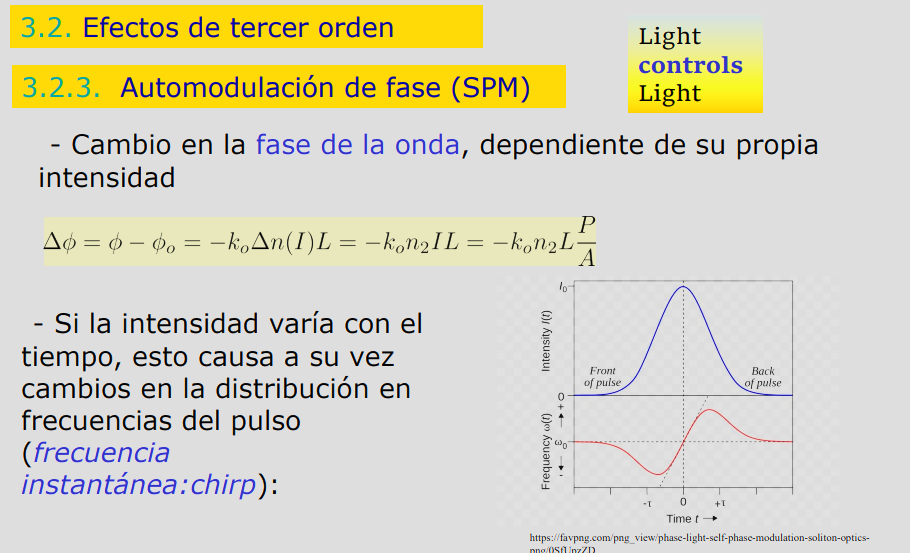
\includegraphics[width=0.7\textwidth]{IMG/tercero17.png}
	\end{figure}

	\esp
	
	Como consecuencia del efecto Kerr óptico, los materiales de tercer orden registran variaciones en la fase de las ondas que se propagan por ellos, y estas variaciones dependen de la intensidad de la propia onda, o bien de la intensidad de una segunda onda que se utilice para cambiar el índice de refracción. Así, este es un caso típico en que puede decirse que la luz controla a la propia luz.
	
	\esp
	
	El cambio de fase introducido para una onda que transporte una potencia $P$ a través de un área $A$ normal a la dirección de propagación es el siguiente:
	
	\esp
	
	\begin{equation}
		\Delta\phi = \phi - \phi_o = -k_o \Delta n(I) L = -k_o n_2 I L = -k_o n_2 L \frac{P}{A}
	\end{equation}
	
	\esp
	
	Por tanto, el proceso se ve favorecido si la longitud del medio es grande y el área transversal del haz pequeña, como puede suceder por ejemplo en una guía de ondas.
	
	\esp
	
	Los procesos de automodulación de fase pueden transformarse en modulación de intensidad utilizando, por ejemplo, un montaje tipo Mach-Zehnder, o bien un medio anisótropo entre dos polarizadores en el que la automodulación de fase varía el retardo entre componentes en el interior del cristal, de forma análoga a lo visto en la sección sobre el efecto Pockels.
	
	\subsubsection{Autoenfoque (SF)}
	
	\begin{figure}[H]
		\centering
		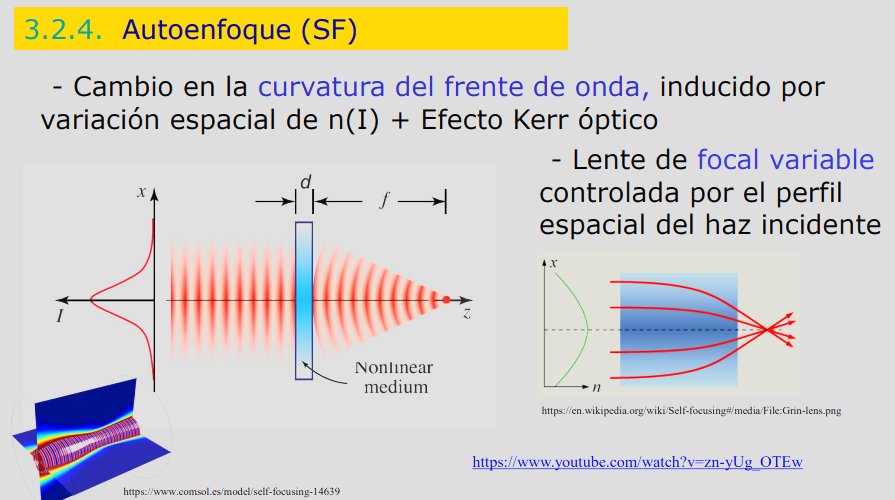
\includegraphics[width=0.7\textwidth]{IMG/tercero18.png}
	\end{figure}
	
	\esp
	
	Si la intensidad de la onda se modula espacialmente, por ejemplo haciendo que sea mayor en el centro del haz, y la onda atraviesa un medio con efecto Kerr óptico, entonces el patrón de variación de índice que se induce en el medio va a parecerse mucho al del perfil de intensidad, ya que $\Delta n(I) = n_2 I$. Esto va a ocasionar un cambio en la curvatura del frente de onda, que puede pasar de plano a esférico.
	
	\esp
	
	Entonces, puede conseguirse de esta forma que el haz focalice en un punto situado detrás del medio, por ejemplo, como se ilustra en la figura. Y además, con la ventaja de que la focal de esta \textit{lente no lineal} puede modularse mediante la intensidad de la propia onda incidente.
	
	\subsubsection{Solitones espaciales}
	
	\begin{figure}[H]
		\centering
		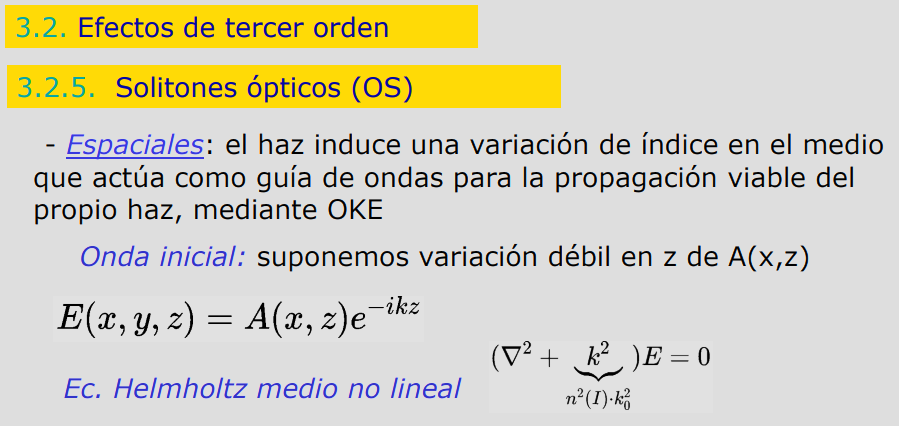
\includegraphics[width=0.7\textwidth]{IMG/tercero19.png}
	\end{figure}
	
	\esp
	
	Siguiendo el principio básico de las aplicaciones descritas antes, pensemos que un pulso que viaja a través de un cierto volumen de medio no lineal presentará en general una distribución de intensidad modulada espacialmente en la sección transversal a la dirección de propagación del pulso (perfil de intensidad). Entonces, esta distribución causará alteraciones en el índice de refracción del medio no lineal por el que viaja, de forma que éste puede considerarse en cierto modo como una guía de onda de índice de refracción variable. Si el perfil de intensidad del pulso es capaz de crear una guía de ondas que permita la propagación del propio pulso de forma estable, entonces el pulso puede propagarse sin alterar espacialmente su forma. Podríamos decir que los efectos de deformación debidos a la difracción son compensados por las variaciones de índice en el propio medio que el haz causa al propagarse por el mismo. El pulso se guía entonces a sí mismo sin apenas distorsiones en su perfil espacial, y se denomina \textit{solitón espacial}.
	
	\esp
	
	También son de gran interés los solitones temporales, en los que la dispersión del medio que causa un incremento en la anchura del pulso es compensada por los efectos no lineales de auto-modulación de fase (SPM) en el mismo, que causan un estrechamiento del pulso, con lo cual el pulso puede viajar por el medio sin deformarse su perfil de modulación temporal.
	
	\esp
	
	Además, cuando se cruzan dos solitones, son capaces de mantener su forma tras la interacción, lo cual resultan muy convenientes en comunicaciones ópticas, para permitir la transmisión de señales a largas distancias sin que la distorsión (espacial o temporal) sea un problema.
	
	\esp
	
	\begin{figure}[H]
		\centering
		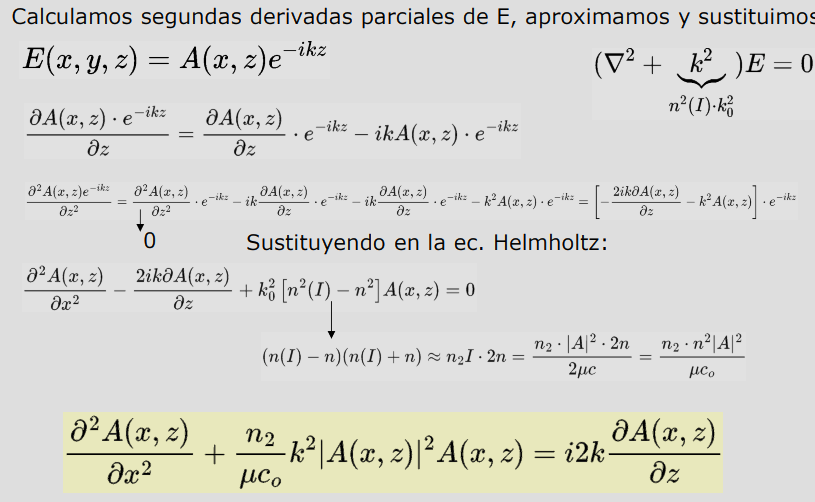
\includegraphics[width=0.7\textwidth]{IMG/tercero20.png}
	\end{figure}
	
	\esp
	
	La forma funcional del pulso puede deducirse considerando una onda inicial $A(x, z) e^{-ikz}$. Utilizando aproximaciones, se puede escribir la ecuación de Helmholtz de esta forma:
	
	\esp
	
	\begin{equation}
		\frac{\partial^2 A(x, z)}{\partial x^2} - i2k \frac{\partial A(x, z)}{\partial z} + k_0^2 \left[ n^2(I) - n^2 \right] A(x, z) = 0
	\end{equation}
	
	\esp
	
	\noindent Considerando que $n_2 I \ll n$, se puede re-escribir la ecuación como:
	
	\esp
	
	\begin{equation}
		\frac{\partial^2 A(x, z)}{\partial x^2} + \frac{n_2}{\mu_0 \epsilon_0} k^2 |A(x, z)|^2 A(x, z) = i2k \frac{\partial A(x, z)}{\partial z}
	\end{equation}
	
	\esp
	
	\begin{figure}[H]
		\centering
		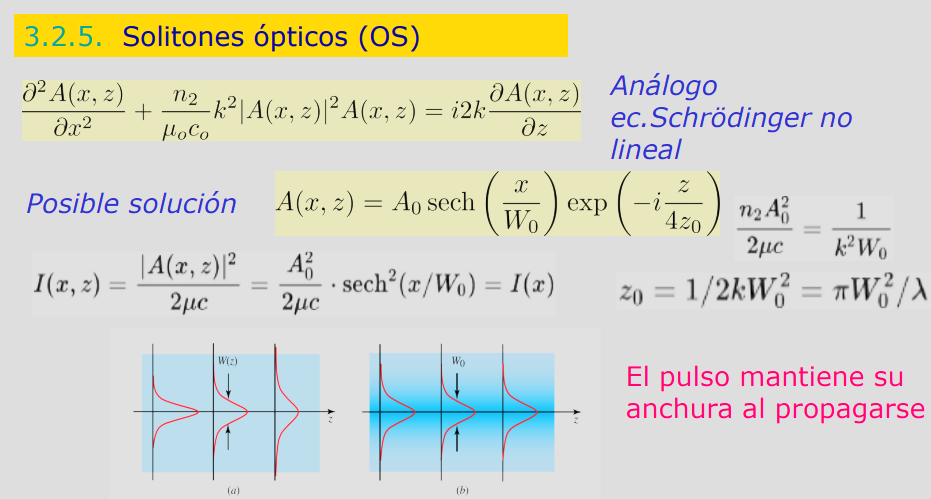
\includegraphics[width=0.7\textwidth]{IMG/tercero21.png}
	\end{figure}
	
	\esp
	
	\noindent Una solución posible para esta ecuación es la función de onda siguiente:
	
	\esp
	
	\begin{equation}
		A(x, z) = A_0 \operatorname{sech} \left( \frac{x}{W_0} \right) \exp \left( -i \frac{z}{4z_0} \right)
	\end{equation}
	
	\esp
	
	con $A_0$ que satisface $n_2 I_0 = \frac{1}{k^2 W_0^2}$, y por tanto el producto $A_0 W_0$ se mantiene constante. Esto se ilustra en la figura 9.
	
	\esp
	
	\begin{figure}[H]
		\centering
		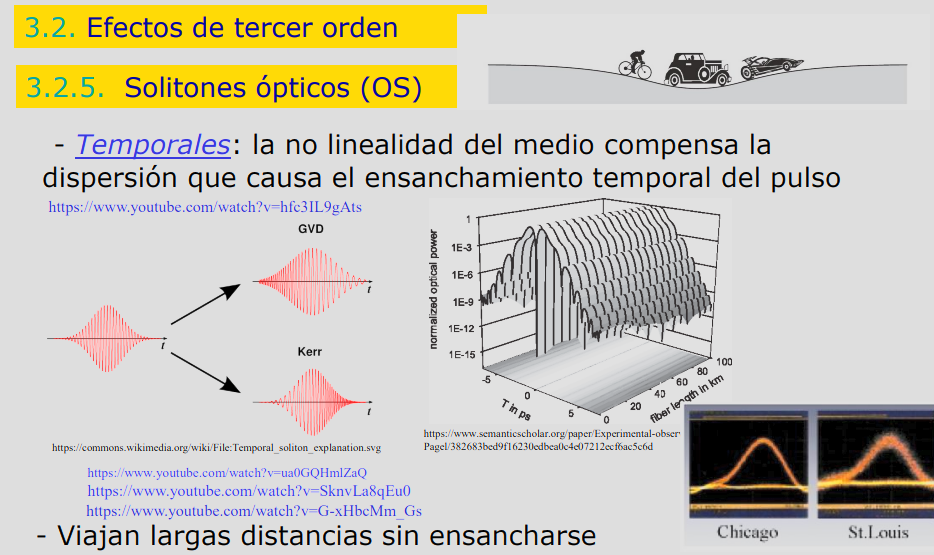
\includegraphics[width=0.7\textwidth]{IMG/tercero22.png}
	\end{figure}
	
	\esp
	
	Una descripción más fundamentada de los solitones temporales puede encontrarse en el capítulo 23 (sección 5) de [1]. De hecho, puede demostrarse que los solitones temporales cumplen una ecuación análoga a la que hemos visto para los solitones espaciales, y en general puede hablarse de una analogía entre ambos; el término solitón muchas veces se aplica a soluciones que cumplen las condiciones necesarias tanto en el dominio espacial (compensando el efecto de ensanchamiento espacial del pulso debido a la dispersión del medio) como en el temporal.
	
	\subsubsection{Modulación de fase cruzada (XPM)}
	
	\begin{figure}[H]
		\centering
		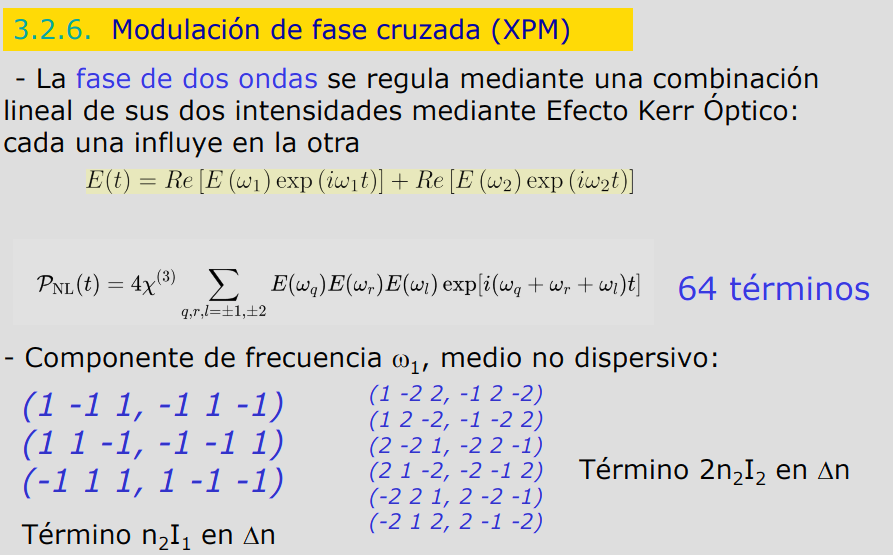
\includegraphics[width=0.7\textwidth]{IMG/tercero23.png}
	\end{figure}
	
	\esp
	
	Este es un fenómeno que ocurre cuando dos ondas de diferente frecuencia se propagan por un medio Kerr. Vamos a partir de la onda incidente, que tendrá la forma:
	
	\esp
	
	\begin{equation}
		E(t) = \text{Re} [E (\omega_1) \exp (i\omega_1 t)] + \text{Re} [E (\omega_2) \exp (i\omega_2 t)]
	\end{equation}
	
	\esp
	
	Sustituyendo esta expresión para la onda incidente en la ecuación $\vec{P}_{NL} = 4\chi^{(3)} \vec{E}^3$, y aislando la componente de frecuencia $\omega_1$, queda:
	
	\esp
	
	\begin{equation}
		P_{NL} (\omega_1) = \chi^{(3)} \left[ 3 |E (\omega_1)|^2 + 6 |E (\omega_2)|^2 \right] E (\omega_1)
	\end{equation}
	
	\esp
	
	\begin{figure}[H]
		\centering
		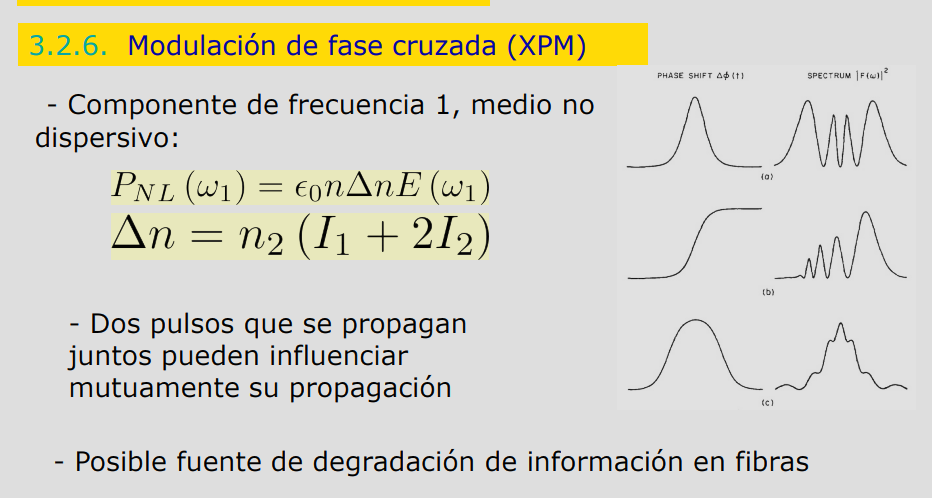
\includegraphics[width=0.7\textwidth]{IMG/tercero24.png}
	\end{figure}
	
	\esp
	
	Asumiendo un medio no dispersivo, de forma que las dos ondas viajen a la misma velocidad, se podría re-escribir la ecuación anterior de la siguiente forma:
	
	\esp
	
	\begin{equation}
		P_{NL} (\omega_1) = \epsilon_0 n \Delta n E (\omega_1)
	\end{equation}
	
	\esp
	
	\noindent siendo $\Delta n = n_2 (I_1 + 2I_2)$.
	
	\esp
	
	Así que la onda de frecuencia $\omega_1$ viaja con un índice de refracción $n + \Delta n$, que depende de su propia intensidad, y también de la intensidad de la onda 2.
	
	\esp
	
	Exactamente el mismo desarrollo puede hacerse para la onda 2, con lo cual la modulación de fase se llama \textit{cruzada}, puesto que ambas ondas influyen la una en la otra de forma similar, y por tanto se pueden considerar como acopladas. Por eso este proceso se llama \textit{modulación de fase cruzada}.
	
	\subsubsection{Mezcla de cuatro ondas (FWM)}
	
	\begin{figure}[H]
		\centering
		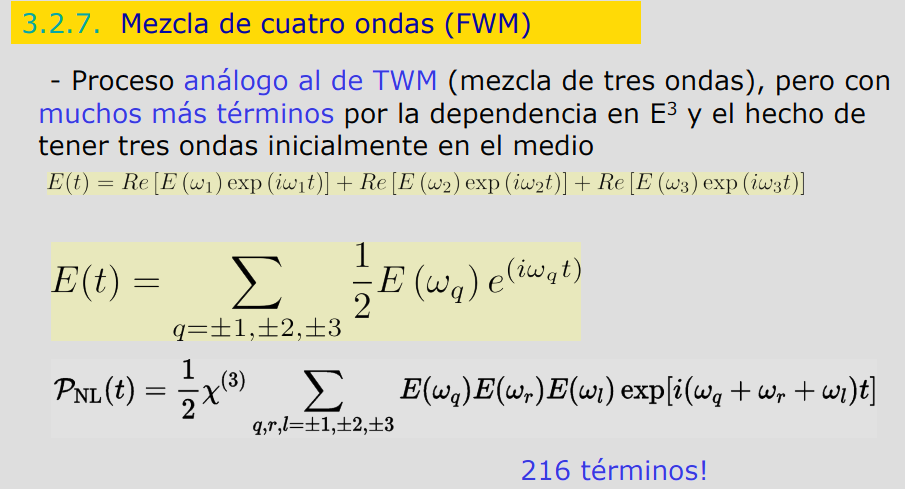
\includegraphics[width=0.7\textwidth]{IMG/tercero25.png}
	\end{figure}
	
	\esp
	
	Los procesos de mezcla de dos ondas no pueden tener lugar tampoco en medios de tercer orden, por las limitaciones señaladas antes para medios de segundo orden, salvo en el caso degenerado. Pero si hay tres ondas propagándose por un medio de tercer orden, pueden generarse nuevas ondas de una forma similar a lo visto para la mezcla de tres ondas, dando lugar a una serie de componentes en frecuencia englobadas dentro del término general de \textit{mezcla de cuatro ondas}, con aplicaciones específicas que vamos a describir en esta subsección, así como las respectivas condiciones de igualación de frecuencia y fase en este caso.
	
	\esp
	
	Consideramos entonces una onda de entrada con tres componentes en frecuencia:
	
	\esp
	
	\begin{equation}
		E(t) = \text{Re} [E (\omega_1) \exp (i\omega_1 t)] + \text{Re} [E (\omega_2) \exp (i\omega_2 t)] + \text{Re} [E (\omega_3) \exp (i\omega_3 t)]
	\end{equation}
	
	\esp
	
	Podemos imaginar la larga serie de términos a los que la sustitución de $E(t)$ en la ecuación de $P_{NL}$ va a dar lugar. Así que es quizá mejor re-escribir $E(t)$ de la siguiente forma:
	
	\esp
	
	\begin{equation}
		E(t) = \sum_{q=\pm 1, \pm 2, \pm 3} \frac{1}{2} E (\omega_q) e^{(i\omega_q t)}
	\end{equation}
	
	\esp
	
	\begin{figure}[H]
		\centering
		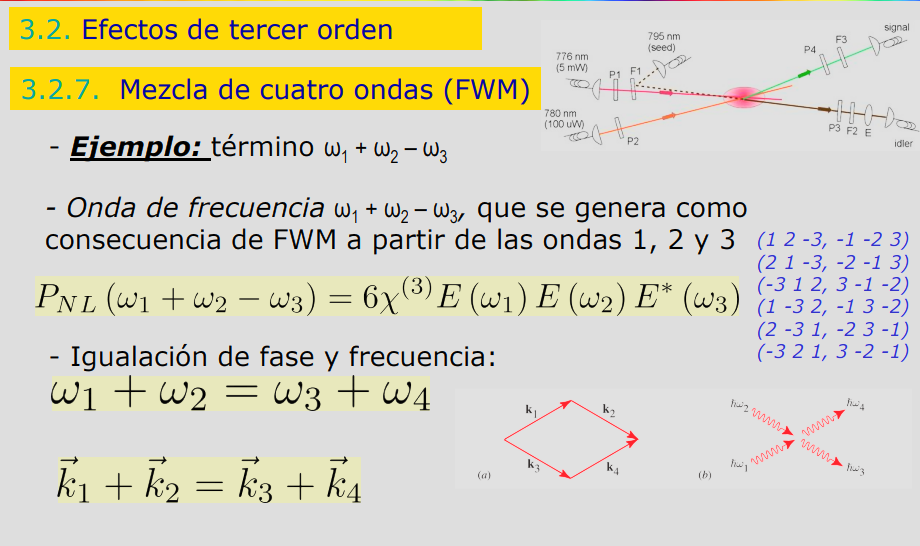
\includegraphics[width=0.7\textwidth]{IMG/tercero26.png}
	\end{figure}
	
	\esp
	
	Adoptamos la convención siguiente: para subíndices $q$ negativos, escribiríamos $E^*(\omega_q) e^{-i\omega_q t}$. Al elevar al cubo este término para calcular $P_{NL}$, obtendremos un total de $6^3 = 216$ términos. Sin embargo, ya que nos interesan las componentes de igual frecuencia y triple producto de amplitudes, podremos agrupar diferentes términos y así podemos deducir las diferentes componentes en frecuencia de $P_{NL}$.
	
	Por ejemplo, en el caso de la componente $P_{NL} (\omega_1 + \omega_2 - \omega_3)$ tendremos que hay seis permutaciones posibles de los términos cruzados que darían lugar a esta frecuencia, luego:
	
	\esp
	
	\begin{equation}
		P_{NL} (\omega_1 + \omega_2 - \omega_3) = 6\chi^{(3)} E (\omega_1) E (\omega_2) E^* (\omega_3)
	\end{equation}
	
	\esp
	
	Este proceso entonces es una mezcla de cuatro ondas, de frecuencias $\omega_1, \omega_2, \omega_3$ y $\omega_4 = \omega_1 + \omega_2 - \omega_3$. Esta última condición puede escribirse de forma alternativa como:
	
	\esp
	
	\begin{equation}
		\omega_1 + \omega_2 = \omega_3 + \omega_4
	\end{equation}
	
	\esp
	
	y constituye la condición de igualación de frecuencia para el proceso de mezcla a cuatro ondas que estamos considerando... la condición de igualación de fase en este caso sería:
	
	\esp
	
	\begin{equation}
		\vec{k}_1 + \vec{k}_2 = \vec{k}_3 + \vec{k}_4
	\end{equation}
	
	\esp
	
	\begin{figure}[H]
		\centering
		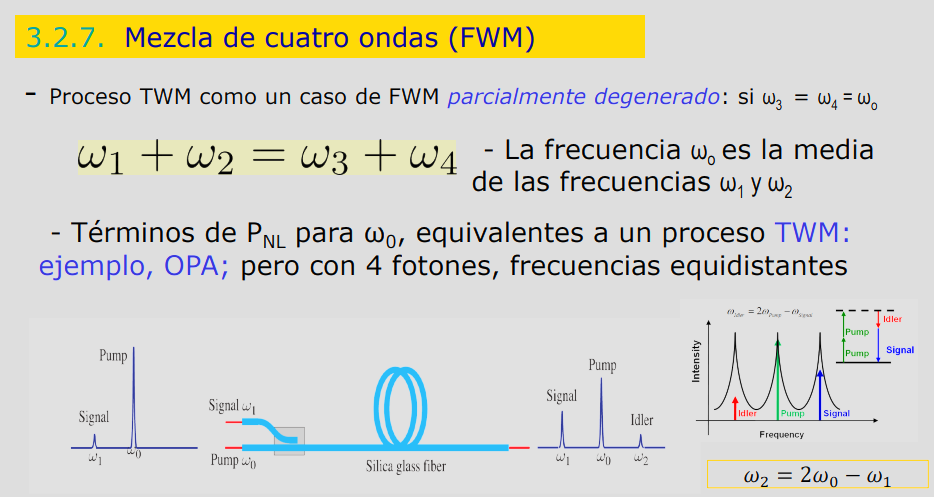
\includegraphics[width=0.7\textwidth]{IMG/tercero27.png}
	\end{figure}
	
	\esp
	
	\noindent \textbf{Mezcla de tres ondas como un proceso FWM degenerado}
	
	\esp
	
	Si dos de las ondas que forman parte del proceso FWM tienen la misma frecuencia (por ejemplo, si las ondas 3 y 4 son de frecuencia $\omega_0$), el proceso de FWM se llama entonces \textit{parcialmente degenerado}. La condición de igualación de frecuencia implica entonces que $\omega_0$ sería la media de las frecuencias $\omega_1$ y $\omega_2$... en la figura 10 se ilustra un proceso de amplificación paramétrica óptica (OPA), pero en este caso sería el resultado de la interacción de cuatro fotones en vez de tres. De forma que dos fotones de la onda de bombeo, de frecuencia $\omega_0$, se aniquilan para dar lugar a un fotón de la frecuencia de la onda señal ($\omega_1$) y otro de la onda idler, cuya frecuencia sería $\omega_2 = 2\omega_0 - \omega_1$.
	
	\esp
	
	\begin{figure}[H]
		\centering
		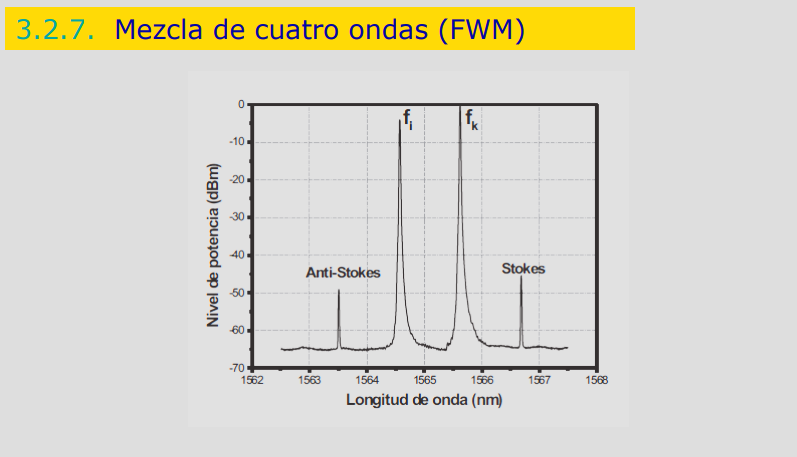
\includegraphics[width=0.7\textwidth]{IMG/tercero28.png}
	\end{figure}
	
	\esp
	
	\begin{figure}[H]
		\centering
		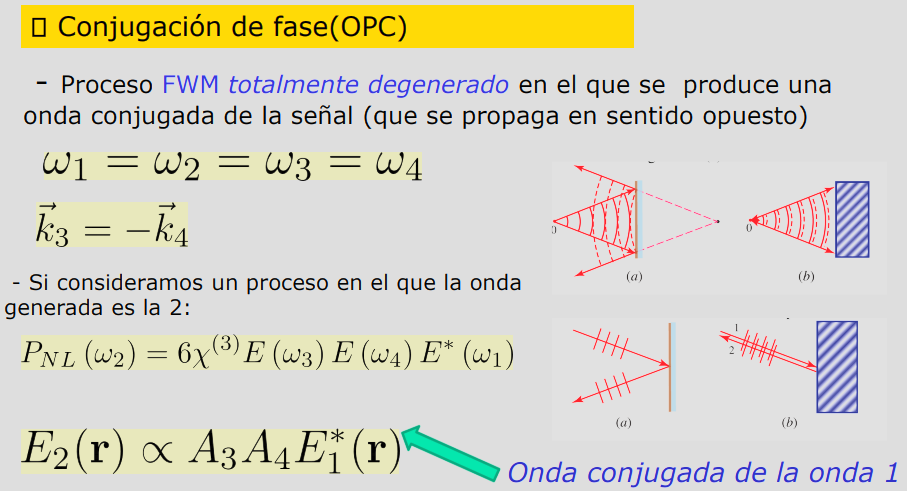
\includegraphics[width=0.7\textwidth]{IMG/tercero29.png}
	\end{figure}
	
	\esp
	
	\textbf{Conjugación de fase óptica (Optical Phase Conjugation, OPC)} Este proceso es un caso de FWM totalmente degenerado, para el cual la frecuencia de las cuatro ondas es la misma. Para el proceso que estamos describiendo, necesitamos además que se cumpla que las ondas 3 y 4 tengan direcciones de propagación opuestas:
	
	\esp
	
	\begin{equation}
		\vec{k}_3 = -\vec{k}_4
	\end{equation}
	
	\esp
	
	Entonces, considerando el término descrito antes para el proceso de mezcla a cuatro ondas en el cual se genera la onda 2:
	
	\esp
	
	\begin{equation}
		P_{NL} (\omega_2) = 6\chi^{(3)} E (\omega_3) E (\omega_4) E^* (\omega_1)
	\end{equation}
	
	\esp
	
	y considerando las ondas 3 y 4 con amplitudes complejas:
	
	\esp
	
	\begin{equation}
		E_3(\mathbf{r}) = A_3 \exp (-j \mathbf{k}_3 \cdot \mathbf{r}), \quad E_4(\mathbf{r}) = A_4 \exp (-j \mathbf{k}_4 \cdot \mathbf{r})
	\end{equation}
	
	\esp
	
	Vemos entonces que se cancelan la parte espacial de la fase en las ondas 3 y 4, quedando finalmente:
	
	\esp
	
	\begin{equation}
		E_2(\mathbf{r}) \propto A_3 A_4 E_1^*(\mathbf{r})
	\end{equation}
	
	\esp
	
	\begin{figure}[H]
		\centering
		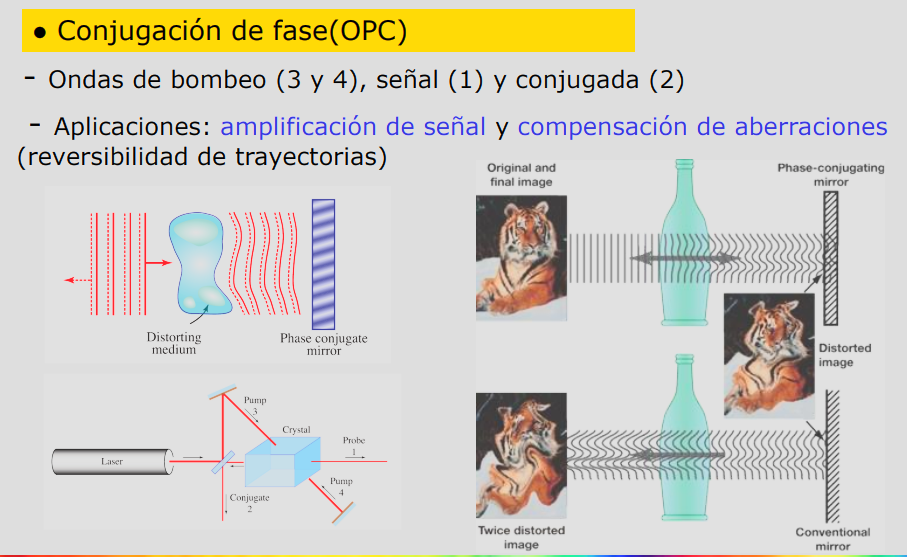
\includegraphics[width=0.7\textwidth]{IMG/tercero30.png}
	\end{figure}
	
	\esp
	
	Que es entonces una onda cuya fase es conjugada de la onda 1. A las ondas 3 y 4 se les llama \textit{ondas de bombeo}, a la onda 1 \textit{sonda o probe} y a la onda 2 \textit{conjugada}. Pero ¿qué características tiene la onda conjugada? Por ejemplo, en el caso de una onda esférica, conjugar la fase equivale a cambiar el signo del exponente en la onda dejando inalterado el resto, de forma que la onda original $\frac{A}{r} e^{-ikr}$, que viaja hacia fuera desde el punto de origen, se convierte en la onda $\frac{A}{r} e^{+ikr}$, que viajaría convergiendo hacia el origen, con la misma amplitud en cada punto del viaje de retorno. En la figura 11, podemos ver el efecto de un espejo normal y uno construido con un medio no lineal que presenta conjugación de fase. Este proceso produce entonces un cambio de sentido sin alterar para nada el frente de onda de la onda incidente.

	
	\esp
	
	La onda conjugada (onda 2 en nuestra notación usual en el proceso de FWM) puede transportar más energía que la onda \textit{sonda o probe}, ya que su intensidad va a ser proporcional al producto de las intensidades de las ondas de bombeo (ondas 3 y 4). Esto hace que los espejos de conjugación de fase puedan convertirse también en amplificadores.
	
	\esp
	
	\begin{figure}[H]
		\centering
		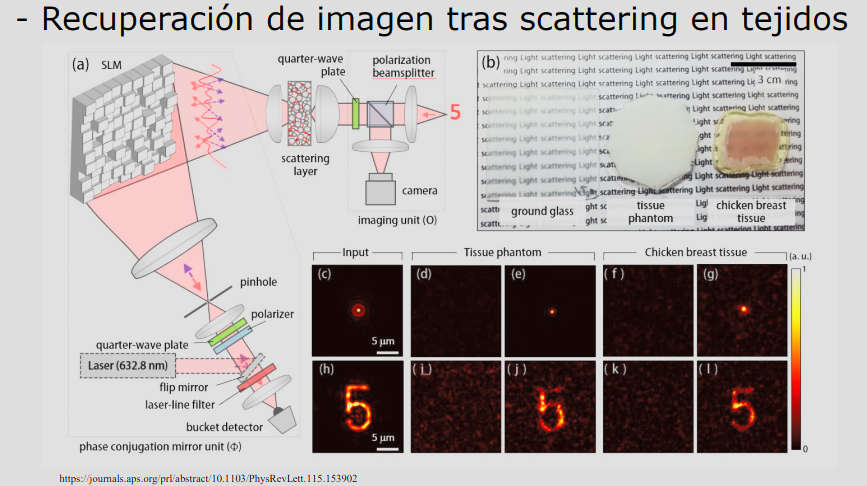
\includegraphics[width=0.7\textwidth]{IMG/tercero31.png}
	\end{figure}
	
	\esp
	
	Es interesante ver la conjugación de fase como un proceso análogo al de inversión temporal (cambio de $t$ por $-t$ en la fase de la onda)... Una aplicación muy destacable del proceso de OPC es la compensación de aberraciones (distorsiones del frente de onda) inducidas por el paso de la luz a través de un medio determinado. Si colocamos un espejo que realice OPC a la derecha del medio que produce las aberraciones, el frente de onda corregirá su distorsión al atravesar dos veces el medio, como podemos ver en la figura 12. El espejo OPC nos asegura que la trayectoria ha sido revertida exactamente.
	
	\esp
	
	En este capítulo, hemos realizado una descripción básica de algunos de los principales fenómenos de Óptica No Lineal... es interesante cuanto menos saber dónde encontrar ampliación de la información básica sobre Óptica No Lineal que hemos podido desarrollar en este tema.

	\printbibliography[title={Bibliografía}]
\end{document}